\documentclass[../main/main.tex]{subfiles}
\begin{document}



%%%%%%%%%%%%%%%%%%%%%%%
%%%%%%%% LECTURE 20 %%%%%%%%
%%%%%%%%%%%%%%%%%%%%%%%

\chapter{Monopoles}

\todo{Qui non ho alcuna bibliografia, se mi suggerisce qualche titolo lo aggiungo volentieri}

The last solitons we will take into account are the monopoles, in particular we will consider general monopoles and t'Hooft-Polyakov monopoles. As usual we start from them classical theory. 

\section{Introduction}

Let us first consider classical electrodynamics in empty space, Maxwell's equations can be written as (we set $c=1$)
\begin{eq}
	\begin{alignedat}{2}
		&\begin{cases}
			\displaystyle-\pder{\vec E}{t}+\vec\nabla\times\vec B=0\\
			\displaystyle\vec\nabla\cdot\vec E=0
		\end{cases}
		&&\quad\leftrightarrow\quad
		\partial_\mu F^{\mu\nu}=0\\
		&\begin{cases}
			\displaystyle \pder{\vec B}{t}+\vec\nabla\times\vec E=0\\
			\displaystyle\vec \nabla\cdot \vec B=0
		\end{cases}
		&&\quad\leftrightarrow\quad
		\lctens^{\mu\nu\rho\sigma}\partial_\nu F_{\rho\sigma=0}
		\quad\leftrightarrow\quad
		\partial_\mu \tilde F^{\mu\nu}=0
	\end{alignedat}
\end{eq}
where $\tilde F$ is the dual of $F$: $\tilde F^{\mu\nu}:=\half\lctens^{\mu\nu\rho\sigma}F_{\rho\sigma}$. 
This system of equations remains unchanged under the replacement
\begin{eq}
	\vec E\mapsto\vec B
	\tcomma
	\vec B\mapsto-\vec E
\end{eq}
or equivalently
\begin{eq}\label{eq:em-duality}
	F_{\mu\nu}\mapsto\tilde F_{\mu\nu}
	\tcomma
	\tilde F_{\mu\nu}\mapsto-F_{\mu\nu}
\end{eq}
Such transformation is called \emph{electromagnetic duality}. However, when we add electric sources via a current $j_e^\mu$ the invariance under duality is broken, because Maxwell's equations become
\begin{eq}\label{eq:Maxw-eqs-current}
	\begin{cases}
		\partial_\mu F^{\mu\nu}=j^\nu_e\\
		\partial_\mu \tilde F^{\mu\nu}=0
	\end{cases}
\end{eq} 
and clearly they are no more invariant under eq.~\eqref{eq:em-duality}. 

\skipline

In 1931 Dirac had the idea to recover the duality invariance introducing also a ``magnetic current'' $j_m^\mu$
\begin{eq}\label{eq:modif-Maxw-eq}
	\begin{cases}
		\partial_\mu F^{\mu\nu}=j^\nu_e\\
		\partial_\mu \tilde F^{\mu\nu}=j^\nu_m
	\end{cases}
\end{eq} 
so that eq.~\eqref{eq:em-duality} still holds provided that under the transformation we exchange the currents $j^\nu_e\leftrightarrow j^\nu_m$. 

However the introduction of the magnetic current raises a problem, since $j_m$ violates the Bianchi identity
\begin{eq}
	\lctens_{\mu\nu\rho\sigma}\partial^\nu F^{\rho\sigma}=0
\end{eq}
that guarantees the global existence of the gauge potential $A_\mu$, 
\begin{eq}
	F^{\mu\nu}=\partial^\mu A^\nu-\partial^\nu A^\mu
\end{eq}
In fact, assume for simplicity the temporal gauge $A^0=0$ and the global existence of $\vec A$. Consider then the zero-component of the second of eq.~\eqref{eq:modif-Maxw-eq}, that is $j_m^0=\partial_\mu \tilde F^{\mu0}=\vec\nabla\cdot\vec B$, and integrate it at a fixed time over a ball $B^3$ containing a magnetic charge. Then we get
\begin{eq}
	Q_m=\int_{B^3}\de^3x\,j_m^0
	=\int_{B^3}\de^3x\,\vec\nabla\cdot\vec B  
	=\oint_{\partial B^3=S^2}\vec B\cdot\de\vec S
	=\oint_{S^2}\vec \nabla\times\vec A\cdot\de \vec S
	=\oint_{\partial S^2=\emptyset}\vec A\cdot \de\vec\ell=0
\end{eq}
hence the magnetic charge associated to $j_m$ should vanish if the gauge potential exists globally.
This problem can be avoided in two ways:
\begin{enumerate}[label=\textbullet]
	\item In the \emph{Wu-Yang approach} we can define $A^\mu$ only on patches (open sets) $\{U_\alpha\}_{\alpha\in A}$ covering $S^2$, then in $U_\alpha\cap U_\beta$ we have $F^{\mu\nu}_\alpha=F^{\mu\nu}_\beta$, $\alpha,\beta\in A$, but $A^\mu_\alpha=A^\mu_\beta+\partial^\mu\lambda_{\alpha\beta}$ for some gauge transformation $\delta A=\partial^\mu\lambda_{\alpha\beta}$. In this way $F^{\mu\nu}$ is still defined globally even if $A^\mu$ isn't, but this is enough in the classical description of physics. 

	\item The other alternative is the one introduced by Dirac, that is the \emph{Dirac string} $j^{\mu\nu}$, introduced in the previous chapter for the quantization of vortices, such that
	\begin{eq}
		F^{\mu\nu}=\partial^\mu A^\nu-\partial^\nu A^\mu+j^{\mu\nu}
	\end{eq}
\end{enumerate}

\subsubsection{The Wu-Yang approach}

Let's make some comments about the Wu-Yang approach (as the Dirac solution has already been discussed in the last chapter).
On the sphere $S^2$ centered on the position of the point-like magnetic charge (\emph{monopole}) we introduce spherical coordinates\footnote{Some relations for spherical coordinates which will be used in the following:
\begin{eq}\label{eq:rel-sph-coord}
	\de\vec x&=\pder{\vec x}r\de r+\pder{\vec x}\theta\de\theta+\pder{\vec x}\varphi\de\varphi
	=\left|\pder{\vec x}{r}\right|\de r\vec e_r+\left|\pder{\vec x}\theta\right|\de\theta\vec e_\theta+\left|\pder{\vec x}{\varphi}\right|\de\varphi\vec e_\varphi
	=\de r\vec e_r+r\de\theta\vec e_\theta+r\sin\theta\de\varphi\vec e_\varphi\\
	%
	\vec\nabla f\cdot\de\vec x&=\pder fr\de r+\pder f\theta\de\theta+\pder f\varphi\de\varphi
	=\pder fr\vec e_r\cdot\de\vec x+\pder f\theta\frac1r\vec e_\theta\cdot\de\vec x+\pder f\varphi\frac1{r\sin\theta}\vec e_\varphi\cdot\de\vec x\\
	%
	\vec\nabla&=\vec e_r\pder{}r+\vec e_\theta\frac1r\pder{}\theta+\vec e_\varphi\frac{1}{r\sin\theta}\pder{}\varphi
\end{eq}
} $(r,\theta,\varphi)$ and define two patches whose union covers $S^2$:
\begin{eq}
	U_1=S^2\setminus\{\theta=\pi\}
	\tcomma
	U_2=S^2\setminus\{\theta=0\}
\end{eq}
On $U_1$ we define
\begin{eq}
	\vec A_1=\frac{Q_m}{4\pi}\frac{\cos\theta-1}{r\sin\theta}\vec e_\varphi
\end{eq}
where $Q_m$ is the magnetic charge and $\vec e_\varphi$ is the unit vector along $\varphi$: in Cartesian coordinates $\vec e_\varphi=(-\sin\varphi,\cos\varphi,0)$. It is clear that $A_1$ is well defined on $S^2$ except for $\theta=\pi$. Analogously on $U_2$ we define
\begin{eq}
	\vec A_2=\frac{Q_m}{4\pi}\frac{\cos\theta+1}{r\sin\theta}\vec e_\varphi
\end{eq}
Let us check that in the intersection of $U_1$ and $U_2$ the gauge potential $A_1$ and $A_2$ differ only by a gauge transformation. 
Writing
\begin{eq}
	\vec A=A_r\vec e_r+A_\theta\vec e_\theta+A_\varphi\vec e_\varphi
\end{eq}
we find
\begin{eq}
	(\vec A_1-\vec A_2)\big|_{U_1\cap U_2}
	=\frac{Q_m}{4\pi}\left[\frac{\cos\theta+1}{r\sin\theta}-\frac{\cos\theta-1}{r\sin\theta}\right]\vec e_\varphi
	=\frac{Q_m}{2\pi}\frac1{r\sin\theta}\vec e_\varphi
	=\frac1{2\pi i}\lexp{-iQ_m\varphi}\vec\nabla \lexp{iQ_m\varphi}
\end{eq}
where in the last line we used eq.~\eqref{eq:rel-sph-coord}. We can also write the last result as ``$\vec\nabla\frac{Q_m}{2\pi}\varphi$'', even if such notation is not completely correct since $\varphi$ is defined up to jumps of $2\pi$. If we compute the magnetic field we get, using $\vec\nabla\times\vec\nabla=0$,
\begin{eq}
	\vec B_1=\vec\nabla\times\vec A_1=\vec \nabla\times\vec A_2=\vec B_2
\end{eq}
so $\vec B$ is globally well defined on $S^2$.
Setting\footnote{Notice that $\vec a$ is the gauge potential with the normalization used in the previous chapter.} $\vec a_j:=2\pi\vec A_j$ we see that $\vec a_1$ is related to $\vec a_2$ in $U_1\cap U_2$ by a well defined $U(1)$ gauge transformation
\begin{eq}
	\lexp{-iQ_m\varphi}\frac{\vec\nabla}i\lexp{iQ_m\varphi}
\end{eq}
with parameter $\lambda_{ij}=Q_m\varphi$. Then also the field strength $F_{ij}$ is globally well defined on $S^2$ and setting $F_{ij}=\frac1{2\pi}f_{ij}$ ($f_{ij}$ turns out to be the curvature of a $U(1)$ connection) we get
\begin{eq}
	\int_{S^2}F_{ij}\de x^i\de x^j=\frac1{2\pi}\int_{S^2} f_{ij}\de x^i\de x^j=Q_m
\end{eq}
which is also called the \emph{first Chern number}. We may also write 
\begin{eq}
	f_{ij}\de x^i\de x^j=\frac{Q_m}2\sin\theta\de\theta\de\varphi=\frac{Q_m}2\frac{1}{r^3}\lctens_{ijk}x^i\de x^j\de x^k
\end{eq} 
which implies
\begin{eq}\label{eq:field-strength-monopole-f}
	f_{ij}=\frac{Q_m}{2}\frac1{r^3}\lctens_{ijk}x^k
	\tso
	f_{ij}^2=\frac{Q_m^2}{4}\frac1{r^6}\lctens_{ijk}\lctens^{ijl}x^kx_l=\frac{Q_m^2}{4}\frac1{r^4}
\end{eq}

\subsubsection{Topological constraints and problems in the quantization}

By choosing $U_1$ as the upper semisphere $S_+^2$ and $U_2$ as the lower semisphere $S_-^2$, then $U_1\cap U_2$ is just the circle in the $z=0$ plane and
\begin{eq}\label{eq:qm-constraint-gauge}
	\int_{S^2}F_{ij}\de x^i\de x^j
	&=\int_{S_+^2}F_{ij}\de x^i\de x^j+\int_{S_-^2}F_{ij}\de x^i\de x^j
	=\int_{S_+^2}\vec\nabla\times\vec A_1\cdot\de\vec\Sigma+\int_{S_-^2}\vec\nabla\times\vec A_2\cdot\de\vec\Sigma\\
	&=\oint_{S^1}(\vec A_1-\vec A_2)\de\vec x
	=\oint_{S^1}\lexp{-iQ_m\varphi}\frac{\vec\nabla}{2\pi i}\lexp{iQ_m\varphi}\de\vec x
	=Q_m\int_0^{2\pi}\frac{\de\varphi}{2\pi}
	=Q_m
\end{eq}
Hence $Q_m$ have a new interpretation, namely it counts how many times the gauge transformation $\lexp{iQ_m\varphi}$ goes around the circle $S^1$ as $\varphi$ goes from $0$ to $2\pi$ (recall that an element of $U(1)$, the gauge group, can be identified with an element of $S^1$). In other words, $\lexp{iQ_m\varphi}\in\pi_1(S^1)\iso\Z$, where $\pi_1$ is again the first homotopy group. The fact that such $U(1)$ map cannot be deformed to a constant guarantees the stability of the monopole. 

\skipline

Up to now the monopole was considered at a fixed time. If we consider a $3+1$ dimensional theory one can quantize the theory, first considering a static monopole with 3 moduli corresponding to the 3 coordinates of the center of the monopole, so that monopole worldlines in a $3+1$ QFT produce line defects. However, in the case of monopoles we have a qualitative difference with respect to kinks and vortices: the energy of the monopole is UV divergent, indeed
\begin{eq}\label{eq:magn-charge-Dirac-monopole}
	\int_{\R^3}\de^3x\,\cenergy
	\sim\int_{\R^3}\de^3x\,F_{ij}^2
	\overset{\eqref{eq:field-strength-monopole-f}}\sim\int_0^\infty \de r\,\frac1{r^2}
	:=\lim_{R\to0}\int_R^\infty\frac{\de r}{r^2}
	=\lim_{R\to0}\frac1R=+\infty
\end{eq}
where $B^3(R)$ denotes a 3-ball of radius $R$ centered on the monopole.  
Since at quantum level the UV divergence of the energy implies divergence in the semi-classical approximation, this suggest that monopoles in the electrodynamical setting are only defined with a UV cutoff, e.g. on a lattice, as we will discuss later on. 

\skipline

Let us show where this singular behaviour of the monopole comes from. One can view this as a consequence of the impossibility of deforming the $U(1)$ transformation $\lexp{iQ_m\varphi}$ to a constant over the circle $S^1$ of arbitrarily small radius, which means that the charge $Q_m$ (which due to eq.~\eqref{eq:qm-constraint-gauge} gives such constraint on the possible deformations) is concentrated in a single point, the center of the monopole. Indeed, the same kind of divergence also appears in the classical description of the electric field, and is due to the localization of the charge of the electron in a point. In the case of the electric field the problem is solved in QFT by replacing the electron with a quantum field, that is an operator valued distribution, which makes sense only when smeared with a test function. 
The problem here is that  in the case of the monopole even the semi-classical approximation is inconsistent, hence we cannot solve this issue as in the case of the electric field. 

\skipline

Consider our $U(1)$ group as a subgroup of $SU(2)$, and recall that a $4\pi$ rotation in $SU(2)$ can be deformed to the identity, since $SU(2)$ is a double cover of $SO(3)$. Suppose that we have a $SU(2)$ gauge theory, instead of the $U(1)$ discussed up to now, in which we are able to construct a solution of the previous equations of motion that behaves like a $U(1)$ monopole of charge 2 at large distances from its center but near the center can explore the entire structure of $SU(2)$. 

In particular, from eq.~\eqref{eq:magn-charge-Dirac-monopole} this means that at high energies (small $r$) the whole structure of the $SU(2)$ group is evident, whereas at low energies (large $r$) only the subgroup $U(1)$ is manifest, that is the $SU(2)$ group structure is ``spontaneously broken'' at low energies, and only the $U(1)$ generator remains unbroken. 

Then the previous argument implying infinite energy would not be valid anymore, since a charge 2 in $U(1)$ is the same as the zero charge in $SU(2)$, so the topological charge in the central point turns out to vanish even if asymptotically we have the structure of a charge 2 monopole. This is the basic idea which leads to the description of the t'Hooft-Polyakov monopole. 

\section{Classical treatment of the t'Hooft-Polyakov monopole}

\cite[Chapter 4]{Shifman:2012}\\

The \emph{t'Hooft-Polyakov monopole} was first introduced in the \emph{Georgi-Glashow model}, which was one of the first attempts to get a unified theory of weak and electromagnetic interactions (now proved to be wrong, but so suggestive that Glashow shared the Nobel prize with the inventors of the Standard Model, Weinberg and Salam). The basic underlying idea was that the $U(1)$ gauge symmetry of QED was just a subgroup of a larger gauge symmetry, $SO(3)$, ``spontaneously broken''\footnote{Here the concept of ``spontaneous symmetry breaking'' apply either perturbatively, in some gauges, or using a non local order parameter, not as in section~\ref{sec:SSB}.} to $U(1)$. By the Anderson-Higgs mechanism the $U(1)$ component of the gauge field create massless photons, whereas the other 2 components, corresponding to the spontaneously broken symmetry, create massive vector mesons $W_\mu^\pm$.\footnote{The $Z^0$ massive uncharged meson was missing: it was introduced in the Standard Model to describe neutral currents, by replacing $SU(3)$ with $SU(2)\times U(1)$.} 

%%%%%%%%%%%%%%%%%%%%%%%
%%%%%%%% LECTURE 21 %%%%%%%%
%%%%%%%%%%%%%%%%%%%%%%%

\skipline

Let's start the description of the Georgi-Glashow model from the fields of the theory. The $SO(3)$ \todo{$SU(2)$?} gauge field is described by 
\begin{eq}
	A:= A_\mu^a\frac{\tau^a}2
	\tfor
	a=1,2,3
	\tand
	\tau^a\  \text{Pauli matrices}
\end{eq}
and its field strength has components
\begin{eq}
	G_{\mu\nu}^a:=\partial_\mu A_\nu^a-\partial_\nu A_\mu^a+\lctens^{abc}A_\mu^bA_\nu^c
\end{eq}
The model contains also a 3-components real scalar field 
\begin{eq}
	\phi:=\phi^a\frac{\tau^a}2
\end{eq}
and its $SO(3)$ covariant derivative is given by 
\begin{eq}
	D_\mu\phi^a:=\partial_\mu\phi^a+\lctens^{abc}A_\mu^b\phi^c
\end{eq}
The Euclidean Lagrangian in $3+1$ dimensions, a kind of non-Abelian generalization of the $2+1$ Higgs model discussed for vortices, is given by
\begin{eq}
	\lag=\frac1{4g^2}(G_{\mu\nu}^a)^2+\half(D_\mu\phi^a)^2+\lambda\big((\phi^a)^2-v^2\big)
\end{eq}
From the action we can derive the following equations of motion
\begin{eq}\label{eq:Georgi-Glashow-eom}
	\begin{cases}
		D_\mu G^{\mu\nu\,a}=-g^2\lctens^{abc}\phi^bD^\nu \phi^c\\
		D_{[\mu}G_{\nu\rho]}^a=0\\
		D_\mu D^\mu\phi^a=4\lambda\phi^a\big((\phi^b)^2-v^2\big)
	\end{cases}
\end{eq}
where the first and the second equations corresponds to the first and the second of eq.~\eqref{eq:Maxw-eqs-current} respectively, and the third correspond to the equation of motion of the scalar field. 

The action is invariant under the following gauge transformations: for $g(x)\in SU(2)$\footnote{Actually the gauge transformations of eq.~\eqref{eq:gauge-transf-georgi-glashow} leave the center of $SU(2)$ invariant, hence they behaves as $SO(3)$ transformations.}
\begin{eq}\label{eq:gauge-transf-georgi-glashow}
	\begin{cases}\begin{aligned}
		A_\mu&\quad\mapsto\quad g^{-1}A_\mu g+g^{-1}\partial_\mu g\\
		\phi&\quad\mapsto\quad g^{-1}\phi g
	\end{aligned}\end{cases}
\end{eq}

\subsubsection{Symmetry breaking boundary conditions}


In order to choose a vacuum configuration, let's impose $SO(3)$ breaking boundary conditions, e.g.
\begin{eq}\label{eq:monopole-boundary-conditions-vacuum}
	\phi^a(\infty)=v\delta^{a3}
	\quad\leftrightarrow\quad
	\phi(\infty)=v\frac{\tau^3}2
\end{eq}
The direction of the vector $\phi^a(\infty)$ in the $SO(3)$ (inducing the $SO(3)$ breaking) can be chosen arbitrarily, but when once it still leaves a $U(1)$ subgroup of $SO(3)$ unbroken, corresponding to rotations around the chosen axis, e.g.
\begin{eq}
	\lexp{i\alpha\frac{\tau^3}2}\underbrace{v\frac{\tau^3}2}_{\phi(\infty)}\lexp{-i\alpha\frac{\tau_3}2}=\underbrace{v\frac{\tau^3}2}_{\phi(\infty)}
\end{eq}
At least perturbatively one often perform a gauge transformation (\emph{unitary gauge}) reducing $\phi=v\frac{\tau^3}2$ everywhere. Then $A_\mu^3$ remains gapless and we identify it with the ``photon field'', whereas
\begin{eq}
	W_\mu^\pm=\frac1{\sqrt2}\frac1g(A_\mu^1\pm iA_\mu^2)
\end{eq}
are the massive vector meson fields. 

\subsubsection{Vacuum sector}

The vacua of the theory are given by the vanishing of all squares in the energy density $\cenergy$. Define the electric and the magnetic field by $G^{a\,0i}=:E^{a\,i}$ and $G^a_{ij}=:-\half\lctens_{ijk}B^{a\,k}$ respectively, then for a static configuration, in the gauge $A_0^a=0$, 
\begin{eq}\label{energy-GG-model}
	\int\de^3\vec x\,\cenergy
	=\int\de^3\vec x\,\bigg[\half\left(\frac{(B^{ai})^2}{g^2}+(D_i\phi^a)^2\right)+\lambda\big((\phi^a)^2-v^2\big)^2\bigg]
\end{eq}
The global minimum of the energy, for the given boundary conditions, is given by
\begin{eq}
	\begin{cases}
		B^a=0\tso A_i^a=g^{-1}\partial_ig\\
		\displaystyle\phi=v\frac{\tau^3}2\\
		D_i\phi^a=0\tso A_i^a=0
	\end{cases}
\end{eq}
where we used the first and the second conditions to obtain the third. 

\subsubsection{Monopoles}

Let's consider the monopole as a static field configuration. First, in order to find the monopole, we want to find the correct ``magnetic field'' of the model. The ``$SO(3)$-magnetic field'' $B_i^a$ is not gauge invariant, hence it is unphysical. But its projections on $\phi$ is gauge invariant, so a natural choice for the ``magnetic field'' is 
\begin{eq}
	B_i^a\frac{\phi^a}{|\phi|}=\half\lctens_{ijk}G_{jk}^a\frac{\phi^a}{|\phi|}
\end{eq}
and its ``magnetic charge'' in units of $g$ can be defined as
\begin{eq}\label{eq:magn-charg-monop}
	Q_m=\lim_{R\to\infty}\frac1g\int_{S_R^2}\de\Sigma^i\, B_i^a\frac{\phi^a}{|\phi|}
\end{eq}

\skipline

We want to find some finite energy configuration with $Q_m\neq0$. From the finiteness of the energy eq.~\eqref{energy-GG-model} as $r\to\infty$ we should have\footnote{The boundary condition eq.~\eqref{eq:monopole-boundary-conditions-vacuum} was imposed in the vacuum configuration.} $(\phi^a(\infty))^2=v^2$ hence at boundaries (described by a sphere $S_\infty^2$ of infinite radius) $\phi$ takes values in a $2$-sphere $S_\phi^2$ of radius $|v|$. 
The continuous maps between these spheres are labelled by an integer $N$ corresponding to an element of the homotopy group $\pi_2(S^2)\iso\Z$, identifying how many times $\phi$ sweeps $S_\phi^2$ when $\vec x$ sweeps $S_\infty^2$. 

Let us consider the case $N=1$, this clearly occours if at $\infty$ we have
\begin{eq}	\label{eq:behav-phi-infty-monopole}
	\phi^a\underset{r\to\infty}\sim v\frac{x^a}{r}=:vn^a
\end{eq}
We see that the group index ``$a$'' is referred to as a group index but also as a spatial index, hence gets ``entangled'' with a coordinate index of $\vec x$ (this is possible since in both cases it runs over 3 components), whereas this would be impossible in $U(1)$). 
Furthermore finiteness of the energy imposes also that as $r\to\infty$ the derivative $D_i\phi^a$ decays faster than $r^{-3/2}$. For eq.~\eqref{eq:behav-phi-infty-monopole} this means that 
\begin{eq}
	\partial_i\phi^a=\partial_i\left(\frac{vx^a}r\right)=\frac vr(\delta^{ai}-n^an^i)\underset{r\to\infty}\sim\frac1r
\end{eq}
which is not enough to satisfy $D_i\phi^a\sim r^{-3/2}$. 
Hence we must choose $A_i^b$ so that
\begin{eq}
	D_i\phi^a=\partial_i\phi^a+\lctens^{abc}A_i^b\phi^c\underset{r\to\infty}\sim O(r^{-3/2})
\end{eq}
This requires 
\begin{eq}\label{eq:A-finite-energy-N-1}
	A_i^a\underset{r\to\infty}\sim\lctens_{aij}\frac{n^j}r
\end{eq}
in fact for such choice of $A_i^a$\footnote{The following identity is needed:
\begin{eq}
\lctens^{ijk}\lctens_{ij'\!k'}=\delta^j_{j'}\delta^k_{k'}-\delta^j_{k'}\delta^k_{j'}
\end{eq}
We will also use
\begin{eq}
	\lctens^{ijk}\lctens_{ijk'}=\delta^k_{k'}
\end{eq}}
\begin{eq}
	\lctens^{abc}A_i^b\phi^c=\lctens^{abc}\lctens^{bij}\frac{n_j}r\frac{x^c}rv=\frac vr(-\delta^{ai}+n^an^i)
\end{eq}
Again, in eq.~\eqref{eq:A-finite-energy-N-1} group and spatial indices are ``entangled''. 

We just obtained that in order to have a finite energy configuration with $Q_m$ non-zero and $N=1$, eq.~\eqref{eq:behav-phi-infty-monopole} and eq.~\eqref{eq:A-finite-energy-N-1} should hold:
\begin{eq}\label{eq:monop-finite-energy-N-1}
	\phi^a\underset{r\to\infty}\sim v\frac{x^a}{r}=vn^a
	\tand
	A_i^a\underset{r\to\infty}\sim\lctens^{aij}\frac{x_j}{r^2}=\lctens^{aij}\frac{n_j}r
\end{eq}
Let us compute $Q_m$ for such configuration using eq.~\eqref{eq:magn-charg-monop}. First notice that
\begin{eq}
	\frac{\phi^a}{|\phi|}B_i^a
	&=\frac{x^a}rB_i^a
	=\frac{x^a}r\left[-\half\lctens_{ijk}(\partial_j A_k^a-\partial_kA_j^a+\lctens^{abc}A_j^bA_k^c)\right]\\
	&=\frac{x^a}r\left[-\lctens_{ijk}\delta^m_j\frac{\lctens^{akm}}{r^2}-\half\lctens_{ijk}\lctens^{abc}\lctens^{bjm}\frac{x_m}{r^2}\lctens^{ckn}{r^2}\right]
	=\frac{x_i}{r^3}
\end{eq}
and then
\begin{eq}
	Q_m&=\lim_{R\to\infty}\frac1g\int_{S_R^2}\de\Sigma^i\, B_i^a\frac{\phi^a}{|\phi|}
	=\lim_{R\to\infty}\frac1g\int_{S_R^2}\de\Sigma^i\, \frac{x_i}{r^3}
	=\lim_{R\to\infty}\frac1g\int_{S_R^2}{r^2\sin\theta\,\de\theta\,\de\varphi}\,\frac{x^i}r\, \frac{x_i}{r^3}
	=\frac{4\pi}g
\end{eq}
and this is exactly the expected \todo{Non mi è ben chiaro come mai questa sia la forma corretta della carica del monopolo.} magnetic charge for a $N=1$ monopole, hence fields as in eq.~\eqref{eq:monop-finite-energy-N-1} are very good candidates for the asymptotic description of the monopole. 

\skipline

In order to find the description of the fields associated to the monopole at finite distances, we introduce the following ansatz, analogous to the one used for the vortices,
\begin{eq}\label{eq:ansatz-tH-P-monop}
	A_i^a=\lctens^{aij}\frac{x_j}{r^2} (1-g_A(r))
	\tcomma
	\phi^a=v\frac{x^a}r(1-g_H(r))
\end{eq}
with $g_A$ and $g_H$ functions vanishing for $r\to\infty$. The requirement that the energy eq.~\eqref{energy-GG-model} is finite as $r\to0$ gives
\begin{eq}
	r^2B^2\underset{r\to0}\sim\frac{1}{r^{1-\epsilon}}
	\tso
	r^2\frac1{r^4}(1-g_A)^2\underset{r\to0}\sim\frac{1}{r^{1-\epsilon}}
\end{eq}
and 
\begin{eq}
	r^2(D_i\phi)^2\underset{r\to0}\sim\frac{1}{r^{1-\epsilon}}
	\tso
	r^2\frac1{r^2}(1-g_H)^2\underset{r\to0}\sim\frac{1}{r^{1-\epsilon}}
\end{eq}
where we used $B\sim\frac1{r^2}(1-g_A)$ and $D_i\phi\sim\frac1{r}(1-g_H)$. Requiring that $B$ and $\phi$ are regular, we obtain
\begin{eq}
	r^2B^2\underset{r\to0}\sim1
	\tso
	r^2\frac1{r^4}(1-g_A)^2\underset{r\to0}\sim1
	\tso
	1-g_A\underset{r\to0}\sim r
\end{eq}
and simultaneously
\begin{eq}
	r^2(D_i\phi)^2\underset{r\to0}\sim1
	\tso
	r^2\frac1{r^2}(1-g_H)^2\underset{r\to0}\sim1
	\tso
	1-g_H\underset{r\to0}\sim 1
\end{eq}
Hence for $1-g_A=O(r)$ and $1-g_H=O(1)$ the solution has finite energy. 

These conditions give a different result for the magnetic charge density respect to the case of the Dirac monopole, indeed
\begin{eq}
	\lim_{R\to0}\frac1g\int_{S_R^2}\de\Sigma^i\, B_i^a\frac{\phi^a}{|\phi|}=0
\end{eq}
so the ``magnetic charge density'' is not concentrated in a point like in the Dirac monopole, and this allows the finiteness of the energy. 
Indeed eq.~\eqref{eq:ansatz-tH-P-monop} give really a static solution of the Georgi-Glashow equations of motion eq.~\eqref{eq:Georgi-Glashow-eom} for $1-g_A=O(r)$ and $1-g_H=O(1)$, and such solution is the (static) t'Hooft-Polyakov monopole. 

\subsubsection{The $\boldsymbol{U(1)}$ symmetry of the monopole}

Recall that a monopole, according to Dirac's description, should be related to a $U(1)$ symmetry. t'Hooft proved that one can define, starting from the non-Abelian field strength $G_{\mu\nu}^a$ of the Georgi-Glashow model, an Abelian $U(1)$ gauge invariant field strength whose singularity is exactly the one of the Dirac monopole. In this way it is possible to see the real monopole structure of the t'Hooft-Polyakov monopole, namely the one corresponding to the Dirac monopole. The correct $U(1)$ ``magnetic field'' found by t'Hooft is obtained by adding to $B_i^a\frac{\phi^a}{|\phi|}$ a contribution vanishing at $\infty$, still gauge invariant, so that instead of the regular structure defined up to now we have the singular structure of the Dirac monopole. 

In order to simplify the notation, let $e^a:=\frac{\phi^a}{|\phi|}$ be the unit vector defined on the points where $|\phi|\neq0$, i.e. outside the center ($r=0$) of the monopole. The $U(1)$ gauge ``magnetic field strength'', $SO(3)$ invariant, proposed by t'Hooft is
\begin{eq}
	F_{\mu\nu}^{U(1)}:=e^a\big[G_{\mu\nu}^a-\lctens^{abc}D_\mu e^b D_\nu e^c\big]
\end{eq}
Indeed, for $|\phi|\neq0$ (brackets are omitted when a derivative acts only on the first element on its side, e.g. $\partial_\mu e^b\partial_\nu e^c=(\partial_\mu e^b)(\partial_\nu e^c)$)
\begin{eq}
	F_{\mu\nu}^{U(1)}
	&=e^a\big[\partial_\mu A_\nu^a-\partial_\nu A_\mu^a+\lctens^{abc}A_\mu^bA_\nu^c-\lctens^{abc}\partial_\mu e^b\partial_\nu e^c-\lctens^{abc}\lctens^{blm}A_\mu^le^m\partial_\nu e^c-\\
	&\qquad-\lctens^{abc}\partial_\mu e^b\lctens^{crs}A_\nu^r e^s-\lctens^{abc}\lctens^{blm}A_\mu^l e^m\lctens^{crs}A_\nu^r e^s\big]\\
	&=e^a\big[\partial_\mu A_\nu^a-\partial_\nu A_\mu^a+\lctens^{abc}A_\mu^bA_\nu^c-\lctens^{abc}\partial_\mu e^b\partial_\nu e^c+A_\mu^a\cancel{e^c\partial_\nu e^c}-A_\mu^ce^a\partial_\nu e^c-\\
	&\qquad-\cancel{\partial_\mu e^be^b}A_\nu^a+\partial_\mu e^bA_\nu^be^a-\lctens^{blm}A_\mu^lA_\nu^ae^me^c+\lctens^{blm}A_\mu^lA_\nu^be^me^a\big]\\
	&=\partial_\mu(e^aA_\nu^a)-\partial_\nu(e^aA_\mu^a)-\lctens^{abc}e^a\partial_\mu e^b\partial_\nu e^c
\end{eq}
where cancellations are due to $e^c\partial_\nu e^c=\half\partial_\nu(e^ce^c)=\half\partial_\nu(1)=0$.
Notice that $e^aA_\mu^a$ is the projection of $A_\mu$ along $\phi$, and $F_{\mu\nu}^{U(1)}$ is defined everywhere, beside in the center of the monopole where $|\phi|=0$. For the monopole solution eq.~\eqref{eq:ansatz-tH-P-monop} we get
\begin{eq}
	e^a=\frac{x^a}r
	\tand
	A_i^ae^a=\cancel{\lctens^{aij}\frac{x^a}r\frac{x_j}{r^2}}(1-g_A(r))=0
\end{eq}
hence
\begin{eq}
	F_{ij}^{U(1)}&=-\lctens^{abc}e^a\partial_\mu e^b\partial_\nu e^c\\
	&=-\lctens^{abc}\frac{x^a}r\partial_i\frac{x^b}r\partial_j\frac{x^c}r\\
	&=-\lctens^{abc}\frac{x^a}{r^3}\partial_i x^b\partial_jx^c
\end{eq}
where in the third line we used the antisymmetry of $\lctens^{abc}$. This result is, up to an overall constant factor, the field strength of the Dirac monopole, eq.~\eqref{eq:field-strength-monopole-f}. Hence $F_{ij}^{U(1)}$ has the same singularity at $r=0$ as in the case of the Dirac monopole, but we obtained it from a finite energy configuration of the Georgi-Glashow model, so at least formally it can be quantized in the continuum. 

\subsubsection{Mass of the monopole}

Let's compute the mass of the classical monopole. This is particularly simple in the case $\lambda=0$ (but still using $\phi^a(\infty)=v\delta^{a3}$ boundary conditions for the vacuum, eq.~\eqref{eq:monopole-boundary-conditions-vacuum}), called \emph{BPS limit}. In this case, in analogy to the Bogomol'nyi treatment of vortices eq.~\eqref{eq:vortex-energy-density-rewritten}, one can rewrite
\begin{eq}
	\int\de^3x\,\cenergy
	=\int\de^3x\,\bigg[\frac1{2g^2}(B_i^a-gD_i\phi^a)^2+\frac1gB_i^aD_i\phi^a\bigg]
\end{eq}
The second term, using the equation of motion $0=D_{[i}G_{jk]}=D_iB_i^a$, can be rewritten as 
\begin{eq}
	\int\de^3x\,\frac1gB_i^aD_i\phi^a=\frac1g\int\de^3x\,\partial_i(B_i^a\phi^a)-\frac1g\int\de^3x\,(\cancel{D_iB_i^a})\phi^a
	=\lim_{R\to\infty}\frac1g\int_{S_R^2}\de\Sigma^i\,B_i^a\phi^a=vQ_m
\end{eq}
Hence if the monopole satisfies $B_i^a=gD_i\phi^a$ as local minimum of the energy, we have
\begin{eq}
	\int\de^3x\,\cenergy=M_m=vQ_m
\end{eq}
This also implies that the t'Hooft-Polyakov monopole in the BPS limit is free and very heavy if $g$ is small. Even if $W^\pm$ mesons described by the Georgi-Glashow model are quite different respect those described by the Standard Model, we may assume that the mass of $W^\pm$ is the same in the two models, and in this case the expected mass of the monopole would be $M_m\sim10\text{TeV}/c^2$ (about the maximum energy reached in the LHC). It has not be found (yet).  

\section{Quantum mechanical treatment of t'Hooft-Polyakov monopole}

\cite[Section 15.5]{Shifman:2012}\\

In the case of the t'Hooft-Polyakov monopole it is important to make some more comments about its quantum mechanical version, since up to now there is no agreed and  well defined QFT description of it. 

The quantum mechanical version of the t'Hooft-Polyakov monopole is obtained promoting the moduli of the the classical solution, corresponding to symmetries broken by the specific choice of the monopole solution, to quantum mechanical (time-dependent) variables. Three moduli correspond to the position of the center of the monopole $\vec x_0$ (up to now $\vec x_0=\vec 0$). There is however a fourth modulus, corresponding to the fact that the ``global''\footnote{Meaning that the symmetry is still described by gauge transformations, but whose group parameters are constant over the whole spacetime.} $U(1)$-electromagnetic symmetry is unbroken, but a fixed monopole solution breaks it. In fact let $e_m(\infty)$ denote the asymptotic behaviour of the normalized scalar field of the monopole. A $U(1)$ transformation of the form $\lexp{i\alpha e_m(x)}$, where $\alpha$ is constant, leaves unchanged the boundary condition of $\phi_m$ (the monopole configuration of the scalar field) but modifies the gauge potential by 
\begin{eq}\label{eq:gauge-pot-alpha-monop}
	A_i\ \mapsto\  A_i^{(\alpha)}:=\lexp{-i\alpha e_m}A_i\lexp{i\alpha e_m}+\frac1i\lexp{-i\alpha e_m}\partial_j\lexp{i\alpha e_m}
\end{eq}
We should consider $\alpha$ as a new modulus associated to the specific monopole solution. Hence in the quantum mechanical treatment 4 time dependent variables $\op{\vec x}_0(t)$ and $\op\alpha(t)$ are introduced, together with their conjugated momenta $\op{\vec p}_0(t)$ and $\op p_\alpha(t)$, and then the quantum mechanical Hamiltonian of the monopole in the quadratic approximation reads
\begin{eq}
	H_m=M_m+\frac{\op{\vec p}_0(t)}{2M_m}+m_W^2\frac{\op p_\alpha^2(t)}{2M_m}
\end{eq}
where the factor $m_W$ is needed since $\alpha$ is an angle, hence $\frac1{2M_m}\op p_\alpha^2$ has not the right dimension in the Hamiltonian. Since $\op\alpha$ is periodic, then $\op p_\alpha$ has discrete spectrum: $\spec(\op p_\alpha)\subseteq\Z$ (for $\hbar=1$).
To understand the meaning of these eigenvalues in the simplest case of a BPS solution, notice that 
\begin{eq}
	\op p_\alpha=\frac{M_m}{m_W^2}\der{\op\alpha}t
\end{eq}
where $m_W^2$ again comes from a dimensional argument, and define the gauge invariant $SO(3)$ electric field for the monopole solution evaluated in the gauge $A_0^a=0$ as
\begin{eq}
	E_i=E_i^a\frac{\phi^a}{|\phi|}=\Tr(E_ie_m)
	\twith 
	E_i=\partial_0A_i^{(\alpha)}
\end{eq}
whose quantum mechanical version is 
\begin{eq}
	\op E_i
	=\Tr\,(\partial_0\op A_i^{(\alpha)}e_m)
	=\der{\op\alpha}t\Tr\,(\partial_\alpha\op A_i^{(\alpha)}e_m)
	\overset{\eqref{eq:gauge-pot-alpha-monop}}=\der{\op\alpha}t\Tr\big(D_i\op e_m\,e_m\big)
\end{eq}
At large distances, since $|\phi|=v$, we can replace $e_m$ by $\frac\phi v$, so that asymptotically
\begin{eq}
	\op E_i
	=\der{\op\alpha}t\frac1v\Tr(D_i\phi\,e_m)
\end{eq}
Then using the BPS equation $B_i^a=D_i\phi^a$ in this limit one can write 
\begin{eq}
	\op E_i
	=\der{\op\alpha}t\frac1{vg}\Tr\,(B_ie_m)
	=\der{\op\alpha}t\frac1{m_W}\Tr\,(B_ie_m)
	=\frac{m_W}{M_m}\op p_\alpha\Tr\,(B_ie_m)
\end{eq}
The electric charge in units of $g$ for the eigenvalue $k\in\Z$ of $\op p_\alpha$ is then given by
\begin{eq}
	Q_e=\lim_{R\to\infty}\frac1g\int_{S_R^2}\de\Sigma^i\,\op E_i
	=\lim_{R\to\infty}\frac1g\int_{S_R^2}\de\Sigma^i\,\frac{m_W}{M_m}k\Tr\,(B_ie_m)
	=\frac1gm_Wk\frac{Q_m}{M_m}
	=k
\end{eq}
where we used $M_m=vQ_m$ and $m_W=vg$. Hence if $k\neq0$ then both $Q_m$ and $Q_e$ are non-vanishing. These solutions, where both electric and magnetic charge are not zero,  are called \emph{dyons}. By consistency, they should appear in the Georgi-Glashow model (meaning that they cannot be removed from the spectrum of the Hamiltonian). 

Hence, while the first three moduli $\vec x_0$ become just the position variables of a quantum mechanical particle, the modulus connected with the symmetry which has been broken by a specific choice of a modulus solution in the internal space is just the information that the spectrum of the theory contains particles with both electric and magnetic charges different from 0. 

%%%%%%%%%%%%%%%%%%%%%%%
%%%%%%%% LECTURE 22 %%%%%%%%
%%%%%%%%%%%%%%%%%%%%%%%

\section{Quantum field theory treatment of Dirac monopoles}

Unfortunately there is no well understood quantum field theory of the 't Hooft-Polyakov monopoles, so in order to discuss a quantum field theory of monopoles we turn again to Dirac monopoles. As previously discussed an UV cutoff is needed for the description of such monopoles, and it is understood in the following of the chapter. However, formally we will write formulas in the continuum notation. 

Again we construct monopole quantum field operators from Euclidean monopole correlators using OS reconstruction. To construct monopole correlation functions it is easier to exploit the duality invariance discussed at the beginning of this chapter: we first construct the correlation functions of charged fields in a scalar electrodynamic without monopoles and then by duality we obtain the Dirac monopole correlators (at least in a theory without electric charges). 

\subsubsection{Strocchi's theorem}

\cite[Chapter 7]{Strocchi_2013}\\

The electric charge in scalar electrodynamic appears as the generator of a global subgroup of a local gauge invariance, this implies an important difference with respect to the topological charges previously discussed. 
Up to now, starting from the correlation functions of the (Euclidean) fields, via reconstruction theorems, we have constructed a Hilbert space of states which was naturally endowed with a positive definite scalar product. 
However for gauge theories, both in the relativistic (such as QED) and non-relativistic cases, the situation is not so simple. The key issue is that a local gauge invariance implies a Gauss' law. 

Let us first consider the problem classically. The Noether's theorem for a global (gauge) invariance yields a conserved current $j_\mu$ using equations of motions (of both the gauge field and the charged field). However, if we mimic its standard proof in the case of local gauge invariance we get the conservation of the current without using the equations of motions of the charged field and the corresponding charge can be determined from measurements at infinity, hence the charge is not local. 

\skipline

To simplify the discussion we consider the Abelian case, a scalar electrodynamic with charged field $\phi$, but the non Abelian case can be treated similarly. In order to simplify the notation we assume unit charge. 

From the gauge invariance of the Lagrangian density 
\begin{eq}
	\lag(\phi,\phi^*,\partial_\mu\phi,\partial_\mu\phi^*,A_\nu,\partial_\mu A_\nu)
\end{eq}
for an infinitesimal gauge transformation parametrized by $\Lambda(x)$
\begin{eq}\label{eq:gauge-tfm-Gauss}
	\delta\phi(x)=i\Lambda(x)\phi(x)
	\tcomma
	\delta\phi^*(x)=-i\Lambda(x)\phi^*(x)
	\tcomma
	\delta A_\mu(x)=-i\partial_\mu\Lambda(x)
\end{eq}
we get
\begin{eq}\label{eq:Noether-proof}
	0&=\delta\lag
	=\fder\lag\phi\delta\phi+\fder\lag{\phi^*}\delta\phi^*+\fder\lag{\partial_\mu\phi}\partial_\mu\delta\phi+\fder\lag{\partial_\mu\phi^*}\partial_\mu\delta\phi^*+\fder\lag{A^\nu}\delta A^\nu+\fder\lag{\partial_\mu A_\nu}\partial_\mu\delta A_\nu\\
	&=i\left[\fder\lag\phi\phi-\fder\lag{\phi^*}\phi^*+\fder\lag{\partial_\mu\phi}\partial_\mu\phi+\fder\lag{\partial_\mu\phi^*}\partial_\mu\phi^*\right]\Lambda+i\left[\fder\lag{\partial_\mu\phi}\phi-\fder\lag{\partial_\mu\phi^*}-\fder\lag{A_\mu}\right]\partial_\mu\Lambda-i\fder\lag{\partial_\mu A_\nu}\partial_\mu\partial_\nu\Lambda
\end{eq}
for $\Lambda(x)$ arbitrary. 
In the case of global symmetry $\Lambda$ is independent on $x$, and using equations of motion of $\phi$ and $\phi^*$
\begin{eq}
	\fder\lag\phi=\partial_\mu\fder\lag{\partial_\mu\phi}
	\tand
	\fder\lag{\phi^*}=\partial_\mu\fder\lag{\partial_\mu\phi^*}
\end{eq}
we get
\begin{eq}
	\partial_\mu\left[\fder\lag{\partial_\mu\phi}\phi-\fder\lag{\partial_\mu\phi^*}\phi^*\right]=0
\end{eq}
so that the Noether current
\begin{eq}\label{eq:Noether-current}
	j^\mu:=\fder\lag{\partial_\mu\phi}\phi-\fder\lag{\partial_\mu\phi^*}\phi^*
\end{eq}
is conserved: $\partial_\mu j^\mu=0$. 

\skipline

But if $\Lambda(x)$ is arbitrary (depending on $x$), also coefficients of $\partial_\mu\Lambda$ and $\partial_\mu\partial_\nu\Lambda$ in eq.~\eqref{eq:Noether-proof} should vanish, hence we have also
\begin{eq}\label{eq:Noether-result-local}
	j^\mu-\fder\lag{A_\mu}=0
	\tand
	\fder\lag{\partial_\mu A_\nu}\partial_\mu\partial_\nu \Lambda=0
\end{eq}
and the latter is satisfied only if 
\begin{eq}
	G^{\mu\nu}:=-\fder\lag{\partial_\mu A_\nu}
\end{eq}
is antisymmetric, $G^{\mu\nu}=G^{[\mu\nu]}$. But then from the first of eq.~\eqref{eq:Noether-result-local} and the equation of motion of $A$ we have
\begin{eq}\label{eq:conserved-curr-em-FS}
	j^\nu=\partial_\mu G^{\mu\nu}
\end{eq}
and due to the antisymmetry of $G^{\mu\nu}$
\begin{eq}
	\partial_\nu j^\nu=\partial_\nu\partial_\mu G^{\mu\nu}=0
\end{eq}
hence $j^\nu$ is automatically conserved without using equations of motion of $\phi$ and $\phi^*$. Moreover, defining the charge
\begin{eq}
	Q:=\int\de^dx\,j^0=\int\de^dx\,\partial_iG^{i0}=\lim_{R\to\infty}\int_{S_R^{d-1}}\!\!\!\de\Sigma_i\,G^{i0}
\end{eq}
associated to $j^\nu$, we see that such global charge does not depend on the local behaviour of the density $j^0$ but only upon the behaviour at infinity of the ``electromagnetic'' field strength $G^{\mu\nu}$. 

\skipline

Since property eq.~\eqref{eq:conserved-curr-em-FS} is a key consequence of the local gauge invariance we must impose it also at quantum level at least in the weakest possible sense, as we are going to see. 

Denote by $\op j_\mu$ and $\op G_{\mu\nu}$ the field operator corresponding to classical $j_\mu$ and $G_{\mu\nu}$, and by $\ket\psi$ and $\ket\chi$ the vectors in the space $\vs$ of states generated by quantum fields of a quantum gauge theory. According to the previous discussion we require that at least in a subspace\footnote{Due to the gauge invariance there are unphysical states, which are elements of $\vs$ but not of $\vsp$.} $\vsp\subseteq\vs$ of physical states the matrix elements satisfy
\begin{eq}
	\bra\psi(\op j^\nu-\partial_\mu \op G^{\mu\nu})(f)\ket\chi=0
	\tfor
	\ket\psi,\ket\chi\in\vsp
\end{eq}
and
\begin{eq}
	\tif 
	\ket\chi\in\vsp
	\tthen
	(\op j^\nu-\partial_\mu\op G^{\mu\nu})(f)\ket\chi\in\vsp
\end{eq}
for a smearing test function $f$ needed in the continuum. Then if $\vs $ has a semi-definite positive inner product, we get the stronger statement
\begin{eq}\label{eq:op-Gauss-law}
	(\op j^\nu-\partial_\mu\op G^{\mu\nu})(f)\ket{\chi}=0
	\tforall
	\ket\chi\in\vsp
\end{eq}
In fact, for $\ket\psi\in\vs$ and $\ket\chi\in\vsp$, using Schwartz inequality
\begin{eq}
	0\leq\vert\bra\psi(\op j^\nu-\partial_\mu\op G^{\mu\nu})(f)\ket\chi\vert^2
	\leq\braket{\psi}{\psi}\underbrace{\bra\chi(\op j^\nu -\partial_\mu \op G^{\mu\nu})^\dagger(f)}_{\in\vsp}(\op j^\nu-\partial_\mu\op G^{\mu\nu})\!\!\!\underbrace{\!\ket\chi\!}_{\in\vsp}=0
\end{eq}
hence eq.~\eqref{eq:op-Gauss-law}, i.e. the Gauss' law as an operator identity, automatically holds in the subspace of physical states. 

\skipline

Let's consider the transformation of the field $\op\phi$, charged with respect to the global gauge group, i.e. (modulo smearings)
\begin{eq}
	0\neq\delta\ophi(y)=[\op Q,\ophi(y)]=\lim_{R\to\infty}\int_{B_R^d}\de^dx[\op j^0(x),\ophi(y)]
\end{eq}
If $\vs$ has a semi-definite inner product and $\ophi(y)$ is local, or at least localized in a bounded region, then for $\ket\psi,\ket\chi\in\vsp$ we have a contraddiction
\begin{eq}
	0\neq\bra\psi\delta\ophi(y)\ket\chi= \bra\psi\lim_{R\to\infty}\int_{B_R^d}\de^dx\,[\op j^0(x),\op\phi(y)]\ket\chi\overset{\eqref{eq:op-Gauss-law}}=\bra\psi\lim_{R\to\infty}\int_{S_R^{d-1}}\de\Sigma_i\,[\op G^{i0}( x),\ophi(y)]\ket\chi=0
\end{eq}
where the vanishing of the commutator is a consequence of locality.

Hence positivity of $\vs$ and locality (in a bounded region) of charged fields are incompatible in a gauge theory. This result in known as \emph{Strocchi's theorem}, and can be rephrased as the impossibility in a gauge theory of having both positivity of the Hilbert space and locality of the charged field.

\skipline

At least formally (neglecting UV problems) the quantity
\begin{eq}\label{eq:op-Q-nonlocal}
	\op Q(\Lambda):=\int\de^3\vec x\,\Lambda(\vec x)(\op j^0(\vec x)-\partial_i \op G^{i0}(\vec x))
\end{eq}
generates the time-independent gauge transformations of parameters $\Lambda(\vec x)$. In fact defining
\begin{eq}
	\delta\ophi(\vec y):=[\op Q(\Lambda),\ophi(\vec y)]
	=\int\de^3\vec x\,\Lambda(\vec x)[\op j^0(\vec x)-\partial_i\op G^{i0}(\vec x),\ophi(\vec y)]
\end{eq}
and using
\begin{eq}
	\op j^0\overset{\eqref{eq:Noether-current}}=(\ophi^*\partial_0\ophi-\ophi\partial_0\ophi^*)
	\tand
	[\partial_0\ophi^*(\vec x),\ophi(\vec y)]=-i\delta(\vec x-\vec y)
\end{eq}
we get
\begin{eq}
	\delta\ophi(\vec y)=\int\de^3\vec x\,\Lambda(\vec x)\ophi(\vec x)\delta(\vec x-\vec y)
	=i\Lambda(\vec y)\ophi(\vec y)
\end{eq}
which coincides with eq.~\eqref{eq:gauge-tfm-Gauss}. Similarly, for the gauge field
\begin{eq}
	\delta \op A_j(\vec y):=[\op Q(\Lambda),\op A_j(\vec y)]
	=\int\de^3\vec x\,\Lambda(\vec x)[-\partial_i\op G^{i0}(\vec x),\op A_j(\vec y)]
	=i\int\de^3\vec x\,\Lambda(\vec x)\partial_i\delta(\vec x-\vec y)\delta_{ij}
	=-i\partial_j\Lambda(\vec y)
\end{eq}

This suggest that if in the reconstruction theorem we use only fields invariant under local gauge transformations ($\delta\ophi=\delta\op A_j=0$) vanishing at infinity, then $\op Q(\Lambda)\vert_{\vsp}=0$ and from eq.~\eqref{eq:op-Q-nonlocal} we get that the Gauss' law is automatically implemented in the reconstructed space of states. If OS positivity holds this must be a Hilbert space, but then charged field operators are non-local, reaching $\infty$ even at fixed time. 

This is not the standard approach based on covariant quantization, gauge-fixing and locality, indeed for the consistency of the monopole, in particular for the unphysical nature of the Dirac string, preserving the gauge invariance appears to be crucial and this approach based on positivity but not locality is the most natural for charged fields.

Therefore we try to get the monopole quantum field starting from a charged non-local quantum field, easier to define, in the electromagnetic dual theory obtained via OS reconstruction from its correlators. Then we apply to these correlators the duality transformation. Let us show how to do this.

\subsubsection{Duality transformation in the path integral}

Notice that in the path integral formalism there is a simple way to derive the duality, starting from the free theory. 

Consider the free photon partition function in the Lorenz gauge\footnote{In the following for simplicity we often don't write explicitly the measure $\de^4x$ in the integrals.}
\begin{eq}\label{eq:duality-free-photon}
	Z_A&=\int\pide A_\mu\,\lexp{-\frac1{2e^2}\int(\partial_{[\mu}A_{\nu]})^2}\delta(\partial^\mu A_\mu)=\\
	&=\text{const}\cdot\int\pide A_\mu^T\,\lexp{-\frac1{2e^2}\int(\partial_{[\mu}A_{\nu]}^T)^2}=\\
	&=\text{const}\cdot\int\pide A_\mu^T\int\pide B_{\mu\nu}\,\lexp{-\frac{e^2}2\int B_{\mu\nu}^2}\,\lexp{i\int B_{\mu\nu}\partial^{[\mu}A_T^{\nu]}}=\\
	&=\text{const}\cdot\int\pide A_\mu^T\int\pide B_{\mu\nu}\,\lexp{-\frac{e^2}2\int B_{\mu\nu}^2}\,\lexp{-i\int (\partial^{[\mu}B_{\mu\nu})A_T^{\nu]}}=\\
	&=\text{const}\cdot\int\pide B_{\mu\nu}\,\lexp{-\frac{e^2}2\int B_{\mu\nu}^2}\,\delta(\partial^{\mu}B_{\mu\nu})\\
\end{eq}
where in the first step we splitted $A_\mu=A_\mu^L+A_\mu ^T$ with $\partial^\mu A_\mu^T=0$ and $\partial^\mu A_\mu=\partial^\mu A_\mu^L$, in the second step we performed a Gaussian transformation with antisymmetric tensor\footnote{Notice that the tensor $B_{\mu\nu}$ plays the role of a Lagrange multiplier.} $B_{\mu\nu}$ (can be checked by integrating over $B_{\mu\nu}$ from the second to the first line), in the third step we integrated by parts in the second exponential, and in the last step we integrated over $A_\mu^T$. 

The constraint $\partial^{\mu}B_{\mu\nu}=0$ can be solved writing $B_{\mu\nu}=\lctens_{\mu\nu\rho\sigma}\partial^\rho\tilde A^\sigma$, for some gauge potential $\tilde A^\sigma$, with possible gauge-fixing $\partial_\mu\tilde A^\mu=0$ which fixes the correspondence $B_{\mu\nu}\leftrightarrow\tilde A_\mu$. In this way the partition function become
\begin{eq}
	Z_A&=\text{const}\cdot\int\pide \tilde A_\mu\,\lexp{-\frac{e^2}2\int (\lctens_{\mu\nu\rho\sigma}\partial^\rho\tilde A^\sigma)^2}\,\delta(\partial^{\mu}\tilde A_\mu)\\
	&=\text{const}\cdot\int\pide \tilde A_\mu\,\lexp{-\frac{e^2}2\int (\partial^{[\rho}\tilde A^{\sigma]})^2}\,\delta(\partial^{\mu}\tilde A_\mu)\\
\end{eq}
Varying with respect to $B_{\mu\nu}$ in the mixed $B_{\mu\nu}$-$A_\mu$ action one finds, using saddle point approximation (which works since the action is quadratic),
\begin{eq}\label{eq:duality_PI}
	\frac ie\partial_{[\mu}A_{\nu]}=eB_{\mu\nu}=\lctens_{\mu\nu\rho\sigma}\partial^\rho\tilde A^\sigma
\end{eq}
(notice that in Minkowski space the first $i$ is missing). We can now construct field strengths of $A$ and $\tilde A$ as follows
\begin{eq}
	F^{\mu\nu}=\partial^{[\mu}A^{\nu]}
	\tand
	\tilde F^{\mu\nu}=\partial^{[\mu}\tilde A^{\nu]}
\end{eq}
which satisfy equations
\begin{eq}
	\partial_\mu F^{\mu\nu}=0
	\quad&\overset{\eqref{eq:duality_PI}}\longleftrightarrow\quad
	\lctens_{\mu\nu\rho\sigma}\partial^\nu\tilde F^{\rho\sigma}=0\\
	\lctens_{\mu\nu\rho\sigma}\partial^\nu F^{\rho\sigma}=0
	\quad&\overset{\eqref{eq:duality_PI}}\longleftrightarrow\quad
	\partial_\mu\tilde F^{\mu\nu}=0
\end{eq}
thus recovering the electromagnetic duality for the free theory. Thus we see how in the free theory the duality arises from a clever change of variables, performing a Gaussian (Fourier) transformation together with the introduction of $B_{\mu\nu}$ and the solution of the constraint on $B_{\mu\nu}$ by means of the field $\tilde A_\mu$. Such procedure is general and can be applied to more general situations.

\subsubsection{The closed defects}

Let us now see how by duality we obtain a theory of electrodynamic with monopoles. We start from the Stückelberg model (for high-energy physics) or the gauged XY model (for condensed matter physics). Under duality monopoles will correspond to the charges of these models. Fields of the model are the angular field $\theta(x)$ and the Abelian gauge field $A_\mu(x)$. The Euclidean Lagrangian is 
\begin{eq}
	\lag=\frac1{2e^2}(\partial_{[\mu}A_{\nu]})^2+\frac\lambda2(-i\lexp{i\theta}\partial_\mu \lexp{i\theta}-A_\mu)^2
\end{eq}
One can write (\emph{Hodge decomposition})
\begin{eq}\label{eq:Hodge-decomp}
	\frac1i\lexp{-i\theta}\partial_\mu \lexp{i\theta}=\partial_\mu\Lambda+2\pi n_\mu
\end{eq}
where $\Lambda$ is real and globally defined and $2\pi n_\mu$ is a singular current corresponding to jumps $0\to2\pi$ in $\theta(x)$, so that $n_\mu(x)\in\Z$. The ``continuity up to jumps of $2\pi$'' of $\theta$ implies\footnote{Let's justify this claim. The function $\theta$ can be regarded as a continuous function with values in $\R$ rather than in $[0,2\pi)$. Then $2\pi n_\mu$ is non-vanishing only in those points where $\theta=2\pi n$ for some $n\in\Z$.} that the singular component $n_\mu$ is non-vanishing only along some lines, therefore it can be regarded as a singular integer valued line-current, that is, a singular integer valued current supported on lines. 

Let's state the Poisson resummation formula: for an angle $\varphi$ we have the Fourier transform
\begin{eq}\label{eq:Poisson-resummation}
	\sum_{n\in\Z}\lexp{-\frac\lambda2(\varphi+2\pi n)^2}=\sum_{j\in\Z}\lexp{-\frac1{2\lambda}j^2}\,\lexp{i\varphi j}
\end{eq}
We can apply its $x$-dependent version to the Lagrangian ($\varphi\mapsto\partial_\mu\Lambda-A_\mu$)
\begin{eq}\label{eq:Poisson-resummation-cont}
	\sum_{n_\mu} \lexp{-\frac\lambda2\int(\partial_\mu\Lambda+2\pi n_\mu-A_\mu)^2}=\sum_{j^\mu}\lexp{-\frac1{2\lambda}\int j_\mu^2}\lexp{i\int(\partial_\mu\Lambda-A_\mu)j^\mu}
\end{eq}
where now $n_\mu(x)$ and $j^\mu(x)$ are integer valued line-currents. In particular $j^\mu$ is the current of charged particles in the Stückelberg model. 
Integration over the scalar field $\Lambda(x)$ gives
\begin{eq}\label{eq:int-Lambda-Poisson}
	\int\pide\Lambda\,\lexp{i\int\de^4x\,(\partial_\mu\Lambda) j^\mu}=\prod_{x\in\R^4}\delta(\partial^\mu j_\mu(x))=:\delta(\partial^\mu j_\mu)
\end{eq}
and $\partial_\mu j^\mu=0$ implies that the support of the current $j_\mu$ is made of closed lines. We see that the term $\exp(-i\int\de^4x\,A_\mu j^\mu)$ describes the world line of a charged particle-antiparticle pair. The closed lines in the support of $j_\mu$ then correspond to boundaries of surfaces. 
%
%%%%%%%%%%%%%%%%%%%%%%%
%%%%%%%% LECTURE 23 %%%%%%%%
%%%%%%%%%%%%%%%%%%%%%%%
%
Let's denote by $S^{\rho\sigma}(x)$ the integer current with support on one of these surfaces for fixed $j_\mu$, so that 
\begin{eq}\label{eq:current-stuck-S}
	j_\mu(x)=\lctens_{\mu\nu\rho\sigma}\partial^\nu S^{\rho\sigma}(x)
\end{eq}
(of course there are many possible choices for the surface, but all these possible choices are equivalent). 

\skipline

The partition function of the Stückelberg model become
\begin{eq}\label{eq:duality-parti-func}
	Z_\lambda
	&=\int\pide A_\mu\int\pide\Lambda\sum_{n_\mu}\,\lexp{-\frac1{2e^2}\int(\partial_{[\mu}A_{\nu]})^2}\lexp{-\frac\lambda2\int(\partial_\mu\Lambda-A_\mu+2\pi n_\mu)^2}\delta(\partial^\mu A_\mu)\\
	&=\int\pide A_\mu^T\int\pide\Lambda\sum_{n_\mu}\,\lexp{-\frac1{2e^2}\int(\partial_{[\mu}A_{\nu]})^2}\lexp{-\frac\lambda2\int(\partial_\mu\Lambda-A_\mu+2\pi n_\mu)^2}\\
	&\overset{\mathclap{\eqref{eq:Poisson-resummation-cont}}}=\int\pide A_\mu^T\int\pide\Lambda\sum_{j_\mu}\,\lexp{-\frac1{2e^2}\int(\partial_{[\mu}A_{\nu]}^T)^2}\,\lexp{-\frac1{2\lambda}\int j_\mu^2}\lexp{i\int (-A_\mu^T+\partial_\mu\Lambda) j^\mu}\\
	&\overset{\mathclap{\eqref{eq:int-Lambda-Poisson}\atop\eqref{eq:current-stuck-S}}}=\,\int\pide A_\mu^T\sum_{S^{\rho\sigma}}\,\lexp{-\frac1{2\lexp2}\int(\partial_{[\mu}A_{\nu]}^T)^2}\,\lexp{-\frac1{2\lambda}\int (\lctens_{\mu\nu\rho\sigma}\partial^\nu S^{\rho\sigma})^2}\lexp{-i\int A^\mu_T\lctens_{\mu\nu\rho\sigma}\partial^\nu S^{\rho\sigma}}\\
	&=\int\pide A_\mu\sum_{S^{\rho\sigma}}\,\lexp{-\frac1{2e^2}\int(\partial_{[\mu}A_{\nu]})^2}\,\lexp{-\frac1{2\lambda}\int (\lctens_{\mu\nu\rho\sigma}\partial^\nu S^{\rho\sigma})^2}\lexp{-i\int A^\mu\lctens_{\mu\nu\rho\sigma}\partial^\nu S^{\rho\sigma}}\delta(\partial^\mu A_\mu)\\
\end{eq}
Applying then the duality procedure as in eq.~\eqref{eq:duality-free-photon} we have 
\begin{eq}
	Z_\lambda&=\int\pide A_\mu^T\int\pide B_{\mu\nu}\sum_{S^{\rho\sigma}}\,\lexp{-\frac{e^2}2\int B_{\mu\nu}^2}\lexp{i\int B_{\mu\nu}\partial^\mu A^\nu_T}\lexp{-\frac1{2\lambda}\int(\lctens_{\mu\nu\rho\sigma}\partial^\nu S^{\rho\sigma})^2}\lexp{-i\int A^\mu_T\lctens_{\mu\nu\rho\sigma}\partial^\nu S^{\rho\sigma}}
\end{eq}
and then integrating out $A_\mu^T$ and taking the limit $\lambda\to\infty$ we get
\begin{eq}
	Z_\infty=\int\pide B_{\mu\nu}\sum_{S^{\rho\sigma}}\lexp{-\frac{e^2}2\int B_{\mu\nu}^2}\delta(\partial^\nu B_{\mu\nu}-\lctens_{\mu\nu\rho\sigma}\partial^\nu S^{\rho\sigma})
\end{eq}
The constraint on $B_{\mu\nu}$ can be solved introducing a gauge field $\tilde A_\mu$ such that
\begin{eq}
	B_{\mu\nu}-\lctens_{\mu\nu\rho\sigma}S^{\rho\sigma}=\lctens_{\mu\nu\rho\sigma}\partial^\rho\tilde A^\sigma
\end{eq}
so that 
\begin{eq}\label{eq:part-func-monop}
	Z_\infty&=\int\pide \tilde A^\mu\sum_{S^{\rho\sigma}}\lexp{-\frac{e^2}2\int(\lctens_{\mu\nu\rho\sigma}(\partial^\rho\tilde A^\sigma+S^{\rho\sigma}))^2}\delta(\partial^\mu\tilde A_\mu)\\
	&=\int\pide\tilde A_\mu\sum_{S^{\rho\sigma}}\lexp{-\frac{e^2}2\int(\partial^{[\rho}\tilde A^{\sigma]}+S^{\rho\sigma})^2}\delta(\partial^\mu\tilde A_\mu)
\end{eq}
If we define the field strength
\begin{eq}
	\tilde{\mathcal F}^{\rho\sigma}=\partial^{[\rho}\tilde A^{\sigma]}+S^{\rho\sigma}
\end{eq}
we see that it satisfies
\begin{eq}
	\lctens_{\mu\nu\rho\sigma}\partial^\nu\tilde{\mathcal F}^{\rho\sigma}=\cancel{\lctens_{\mu\nu\rho\sigma}\partial^\nu\partial^{[\rho}\tilde A^{\sigma]}}+\lctens_{\mu\nu\rho\sigma}\partial^\nu S^{\rho\sigma}\overset{\eqref{eq:current-stuck-S}}=j_\mu
\end{eq}
This proves that $j^\mu$ are monopole currents with respect to $\tilde A^\mu$, i.e. the worldlines of monopole-antimonopole pairs. 
Accordingly $S^{\rho\sigma}$ should describe the 2-dimensional worldsheet spanned by the Dirac string between the monopole and the antimonopole of the pair. The arbitrariness of the choice of $S^{\rho\sigma}$ reflects the arbitrariness of the Dirac string. Hence monopole currents are the locus of the defects in the electrodynamics of the monopoles. 

\subsubsection{Open defects and correlators}

Let us see how to ``open'' such line defects using duality. A charged gauge-invariant non-local field in the Stückelberg model can be constructed using a recipe suggested by Dirac in the operator setting (for QED), adapted to the path-integral formalism. 

The charged field of the Stückelberg model (given by quantization of the complex field $\phi$ with $|\phi|=1$) is $\lexp{i\op\theta(\vec x)}$, clearly not-gauge invariant under the gauge transformation
\begin{eq}
	\lexp{i\op\theta(\vec x)}\quad\to\quad \lexp{i(\op\theta(\vec x)+e\Lambda(\vec x))}
\end{eq}
Dirac suggested\footnote{The idea of Dirac, qualitatively, it that an electron, even asymptotically, carries with it also its Coulomb field, hence when an electron is created its Coulomb field should be created as well. Applying this idea to the scalar field (rather than to the electron field) we get the procedure we are describing in the following.} to make it gauge invariant multiplying it by
\begin{eq}
	\lexp{ie\int\de^3\vec y\, E_i^{\vec x}(\vec y)\op A^i(\vec y)}
\end{eq}
where $\op A^i$ is the gauge potential of the quantum ``photon'' field and $E_i^{\vec x}$ denote the (classical) electric field generated by a unit charge at the position $\vec x$, so that by the classical Gauss' law
\begin{eq}
	\partial^iE_i^{\vec x}(\vec y)=\delta(\vec x-\vec y)
\end{eq}
In fact, under a gauge transformation $\Lambda(\vec x)$ vanishing at $\infty$
\begin{eq}
	\lexp{ie\int\de^3\vec y\, E_i^{\vec x}(\vec y)\op A^i(\vec y)}
	\quad\to\quad
	&\lexp{ie\int\de^3\vec y\, E_i^{\vec x}(\vec y)(\op A^i(\vec y)+\partial_i\Lambda(\vec y))}=\\
	&\quad=\lexp{ie\int\de^3\vec y\,E_i^{\vec x}(\vec y)\op A_i(\vec y)}\lexp{-ie\int\de^3\vec y\,\partial^i E_i^{\vec x}(\vec y)\Lambda(\vec y)}=\\
	&\quad=\lexp{ie\int\de^3\vec y\,E_i^{\vec x}(\vec y)\op A_i(\vec y)}\lexp{-ie\Lambda(\vec x)}
\end{eq}
so that 
\begin{eq}\label{eq:Dirac-recipe-quant}
	\lexp{i\op\theta(\vec x)}\lexp{ie\int\de^3\vec y\, E_i^{\vec x}(\vec y)\op A^i(\vec y)}
\end{eq}
is gauge invariant but still charged, hence it is physical and should be added to the Hilbert space of the theory due to completeness. The second term in eq.~\eqref{eq:Dirac-recipe-quant} describes the Coulomb field always attached to a charged particle.

It is easy to define the corresponding Euclidean field (now in $\R^4$). Define
\begin{eq}
	E_i^{ x}( y)=\delta(x^0-y^0)E_i^{\vec x}(\vec y)
	\tcomma
	E_o^x(y)=0
\end{eq}
then the charged non-local Euclidean field is given by 
\begin{eq}
	\lexp{i\theta(x)}\lexp{ie\int\de^4y\,E_\mu^x(y)A^\mu(y)}
\end{eq}
The Euclidean correlator of such fields naturally satisfy the OS positivity, hence using the OS reconstruction it is possible to obtain a charged quantum field operator (in the lattice). 

However we are interested in the quantum field operator for the monopole, so let's apply the duality transformation to
\begin{eq}\label{eq:exp-value-monopole-duality}
	\big\langle \lexp{i\theta(x)}\lexp{ie\int\de^4z\,E_\mu^x(z)A^\mu(z)}\lexp{-i\theta(y)}\lexp{-ie\int\de^4w\,E_\mu^y(w)A^\mu(w)}\big\rangle_\lambda
\end{eq}
where $\langle\quad\rangle_\lambda$ denotes the expectation value in the model with the fixed value $\lambda$.
To apply the duality transformation we need to re-express the $\theta$-dependence appearing in the expectation value in terms of $\frac1i\lexp{-i\theta}\partial_\mu \lexp{i\theta}=\partial_\mu\Lambda+2\pi n_\mu$. This can be achieved introducing a current $j_\mu^{xy}$ satisfying
\begin{eq}
	\partial^\mu j_\mu^{xy}(w)=\delta(y-w)-\delta(x-w)
\end{eq}
using this current we can write
\begin{eq}
	\lexp{\int\de^4w\,j_\mu^{xy}(w)\lexp{-i\theta(w)}\partial^\mu \lexp{i\theta(w)}}
	&=\lexp{\int\de^4w\,j_\mu^{xy}(w)\partial_\mu\log \lexp{i\theta(w)}}
	=\lexp{-\int\de^4w\,\partial^\mu j_\mu^{xy}(w)\log \lexp{i\theta(w)}}\\
	&=\lexp{-\log \lexp{i\theta(y)}+\log \lexp{i\theta(x)}}
	=\lexp{i(\theta(x)-\theta(y))}
\end{eq}
so our 2-point function eq.~\eqref{eq:exp-value-monopole-duality} according to the decomposition eq.~\eqref{eq:Hodge-decomp} becomes
\begin{eq}
	&\langle \lexp{i\theta(x)}\lexp{ie\int\de^4z\,E_\mu^x(z)A^\mu(z)}\lexp{-i\theta(y)}\lexp{-ie\int\de^4w\,E_\mu^y(w)A^\mu(w)}\rangle_\lambda=\\
	&\qquad=\langle \lexp{ie\int\de^4w\,(E_\mu^x(w)-E_\mu^y(w))A^\mu(w)}\lexp{i\int\de^4w\,j_\mu^{xy}(w)(\partial^\mu\Lambda+2\pi n^\mu)(w)}\rangle_\lambda
\end{eq}
Note that 
\begin{eq}
	\lexp{i\int\de^4w\,j_\mu^{xy}(w)2\pi n^\mu(w)}=1
\end{eq}
since both $j_\mu^{xy}$ and $n_\mu$ are integer valued, hence we get
\begin{eq}
	&\langle \lexp{i\theta(x)}\lexp{ie\int\,E_\mu^xA^\mu}\lexp{-i\theta(y)}\lexp{-ie\int\,E_\mu^yA^\mu}\rangle_\lambda=\\
	&\qquad=\frac1{Z_\lambda}\int\pide A_\mu\int\pide\Lambda\sum_{n_\mu}\,\lexp{ie\int\,(E_\mu^x-E_\mu^y)A^\mu}\lexp{i\int\,j_\mu^{xy}\partial^\mu\Lambda}\lexp{-\frac1{2e^2}\int(\partial_{[\mu}A_{\nu]})^2}\lexp{-\frac\lambda2\int(\partial_\mu\Lambda-A_\mu+2\pi n_\mu)^2}\delta(\partial^\mu A_\mu)\\
	&\qquad\overset{\mathclap{\eqref{eq:Poisson-resummation-cont}}}=\,\frac1{Z_\lambda}\int\pide A_\mu\int\pide\Lambda\sum_{j_\mu}\,\lexp{ie\int\,(E_\mu^x-E_\mu^y)A^\mu}\lexp{i\int\,j_\mu^{xy}\partial^\mu\Lambda}\lexp{-\frac1{2e^2}\int(\partial_{[\mu}A_{\nu]})^2}\lexp{-\frac1{2\lambda}\int j_\mu^2}\lexp{i\int(\partial_\mu\Lambda-A_\mu)j^\mu}\delta(\partial^\mu A_\mu)\\
	&\qquad\overset{\mathclap{\eqref{eq:int-Lambda-Poisson}}}=\ \frac1{Z_\lambda}\int\pide A_\mu\sum_{j_\mu}\,\lexp{ie\int\,(E_\mu^x-E_\mu^y)A^\mu}\lexp{-\frac1{2e^2}\int(\partial_{[\mu}A_{\nu]})^2}\lexp{-\frac1{2\lambda}\int j_\mu^2}\lexp{-i\int A_\mu j^\mu}\delta(\partial^\mu j_\mu+\partial^\mu j_\mu^{xy})\delta(\partial^\mu A_\mu)\\
\end{eq}
hence $\partial^\mu j_\mu(w)=-\partial^\mu j_\mu^{xy}(w)=\delta(w-x)-\delta(w-y)$, or equivalently $\partial^\mu j_\mu=\delta_x-\delta_y$, where we defined $\delta_x(w):=\delta(w-x)$. 
Finally in the limit $\lambda\to\infty$, which we have seen is dual to the electrodynamic with monopoles, the correlation function becomes\todo{C'è un problema con la carica $e$, a volte è omessa e altre no.}
\begin{eq}\label{eq:monop-correlat-lambda-infty}
	&\langle \lexp{i\theta(x)}\lexp{ie\int\de^4z\,E_\mu^x(z)A^\mu(z)}\lexp{-i\theta(y)}\lexp{-ie\int\de^4w\,E_\mu^y(w)A^\mu(w)}\rangle_\infty=\\
	&\qquad=\frac1{Z_\infty}\int\pide A_\mu\,\lexp{-\frac1{2e^2}\int(\partial_{[\mu}A_{\nu]})^2}\delta(\partial^\mu A_\mu)\sum_{\scriptstyle j_\mu\atop\scriptstyle\partial^\mu j_\mu=\delta_x-\delta_y}\lexp{i\int A_\mu(-j_\mu+E_\mu^x-E_\mu^y)}=\\
	&\qquad=\frac1{Z_\infty}\int\pide A_\mu\,\lexp{-\frac1{2e^2}\int(\partial_{[\mu}A_{\nu]})^2}\delta(\partial^\mu A_\mu)\sum_{\scriptstyle j_\mu\atop\scriptstyle\partial^\mu j_\mu=0}\lexp{i\int A_\mu(-j_\mu+j_\mu^{xy}+E_\mu^x-E_\mu^y)}\\
\end{eq}
The situation is represented in fig.~\ref{fig:monop-correlator}.
%
\begin{figure}[h]
\centering

\tikzset{every picture/.style={line width=0.75pt}} %set default line width to 0.75pt
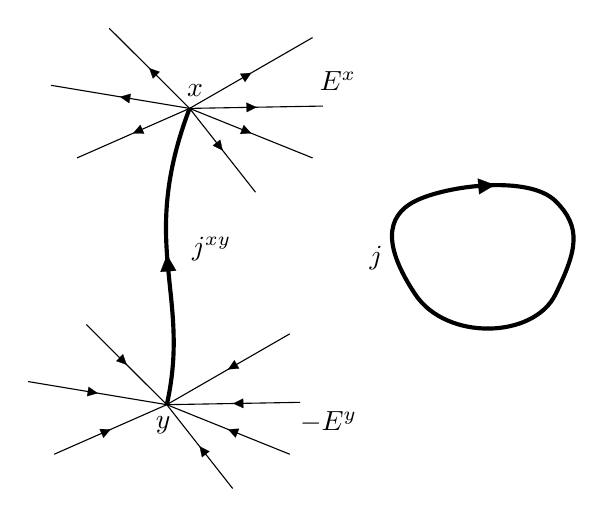
\begin{tikzpicture}[x=0.75pt,y=0.75pt,yscale=-0.75,xscale=0.75]

%Curve Lines [id:da34763408485182423] 
\draw [line width=1.5]    (215.33,247.83) .. controls (231.33,177.08) and (196.5,145.75) .. (230,57.5) ;
\draw [shift={(215.49,151.69)}, rotate = 445.45] [fill=black][line width=0.08] (10.45,-5.02) -- (0,0) -- (10.45,5.02) -- cycle    ;
%Straight Lines [id:da9536377690303859] 
\draw (230,57.5) -- (309,89.33) ;
\draw [shift={(269.5,73.42)}, rotate = 201.95] [fill=black][line width=0.08] (6.25,-3) -- (0,0) -- (6.25,3) -- cycle    ;
%Straight Lines [id:da5956258746113772] 
\draw (230,57.5) -- (309,12) ;
\draw [shift={(269.5,34.75)}, rotate = 510.06] [fill=black][line width=0.08] (6.25,-3) -- (0,0) -- (6.25,3) -- cycle    ;
%Straight Lines [id:da40651481967876824] 
\draw (141,42.67) -- (230,57.5) ;
\draw [shift={(185.5,50.08)}, rotate = 9.46] [fill=black][line width=0.08] (6.25,-3) -- (0,0) -- (6.25,3) -- cycle    ;
%Straight Lines [id:da20641993760547628] 
\draw (178.33,6) -- (230,57.5) ;
\draw [shift={(204.17,31.75)}, rotate = 44.91] [fill=black][line width=0.08] (6.25,-3) -- (0,0) -- (6.25,3) -- cycle    ;
%Straight Lines [id:da12391154990815179] 
\draw (157.67,89.33) -- (230,57.5) ;
\draw [shift={(193.83,73.42)}, rotate = 336.25] [fill=black][line width=0.08] (6.25,-3) -- (0,0) -- (6.25,3) -- cycle    ;
%Straight Lines [id:da21526296373902576] 
\draw (230,57.5) -- (315.67,56) ;
\draw [shift={(272.83,56.75)}, rotate = 539] [fill=black][line width=0.08] (6.25,-3) -- (0,0) -- (6.25,3) -- cycle    ;
%Straight Lines [id:da8937832289395333] 
\draw (230,57.5) -- (272.33,111.33) ;
\draw [shift={(251.17,84.42)}, rotate = 231.82] [fill=black][line width=0.08] (6.25,-3) -- (0,0) -- (6.25,3) -- cycle    ;
%Straight Lines [id:da9575622782574718] 
\draw (215.33,247.83) -- (294.33,279.67) ;
\draw [shift={(254.83,263.75)}, rotate = 21.95] [fill=black][line width=0.08] (6.25,-3) -- (0,0) -- (6.25,3) -- cycle    ;
%Straight Lines [id:da6034055373922615] 
\draw (215.33,247.83) -- (294.33,202.33) ;
\draw [shift={(254.83,225.08)}, rotate = 330.06] [fill=black][line width=0.08] (6.25,-3) -- (0,0) -- (6.25,3) -- cycle    ;
%Straight Lines [id:da15166429129257053] 
\draw (126.33,233) -- (215.33,247.83) ;
\draw [shift={(170.83,240.42)}, rotate = 189.46] [fill=black][line width=0.08] (6.25,-3) -- (0,0) -- (6.25,3) -- cycle    ;
%Straight Lines [id:da3975888310879898] 
\draw (163.67,196.33) -- (215.33,247.83) ;
\draw [shift={(189.5,222.08)}, rotate = 224.91] [fill=black][line width=0.08] (6.25,-3) -- (0,0) -- (6.25,3) -- cycle    ;
%Straight Lines [id:da004602224665434473] 
\draw (143,279.67) -- (215.33,247.83) ;
\draw [shift={(179.17,263.75)}, rotate = 516.25] [fill=black][line width=0.08] (6.25,-3) -- (0,0) -- (6.25,3) -- cycle    ;
%Straight Lines [id:da6747402885776581] 
\draw (215.33,247.83) -- (301,246.33) ;
\draw [shift={(258.17,247.08)}, rotate = 359] [fill=black][line width=0.08] (6.25,-3) -- (0,0) -- (6.25,3) -- cycle    ;
%Straight Lines [id:da7626517334341056] 
\draw (215.33,247.83) -- (257.67,301.67) ;
\draw [shift={(236.5,274.75)}, rotate = 51.82] [fill=black][line width=0.08] (6.25,-3) -- (0,0) -- (6.25,3) -- cycle    ;
%Shape: Polygon Curved [id:ds005057235324020137] 
\draw [line width=1.5]  (375,117) .. controls (395,107) and (448,100.17) .. (465,117) .. controls (482,133.83) and (479,148.5) .. (465,177) .. controls (451,205.5) and (395,207) .. (375,177) .. controls (355,147) and (355,127) .. (375,117) -- cycle ;
%Straight Lines [id:da26027023119900883] 
%\draw [line width=1.5]    (351.33,113.5) -- (422.02,107.03) ;
\draw [shift={(426,106.67)}, rotate = 534.77] [fill=black][line width=0.08] (10.45,-5.02) -- (0,0) -- (10.45,5.02) -- cycle    ;

% Text Node
\draw (226.67,40.73) node [anchor=north west][inner sep=0.75pt]    {$x$};
\draw (206.67,253.73) node [anchor=north west][inner sep=0.75pt]    {$y$};
\draw (312,32.4) node [anchor=north west][inner sep=0.75pt]    {$E^x$};
\draw (299.33,250.73) node [anchor=north west][inner sep=0.75pt]    {$-E^y$};
\draw (230,138.4) node [anchor=north west][inner sep=0.75pt]    {$j^{xy}$};
\draw (344,144.4) node [anchor=north west][inner sep=0.75pt]    {$j$};
\end{tikzpicture}
%
\caption{Representation of currents and fields in eq.~\eqref{eq:monop-correlat-lambda-infty} in one dimension less.}
\label{fig:monop-correlator}
\end{figure}

Since $\partial^\mu(j_\mu^{xy}+E_\mu^x-E_\mu^y)=0$, it exists a tensor $S^{\rho\sigma}(z|j^{xy},E^x,E^y)$ such that
\begin{eq}
	-(j_\mu^{xy}+E_\mu^x-E_\mu^y)(z)=\lctens_{\mu\nu\rho\sigma}\partial^\nu S^{\rho\sigma}(z|j^{xy},E^x,E^y)
\end{eq}
Using the Hodge decomposition one can give a more explicit expression for this tensor
\begin{eq}
	S^{\rho\sigma}(z|j^{xy},E^x,E^y)=\int\de w\,\lctens^{\rho\sigma\alpha\beta}\partial_\alpha\Delta^{-1}(z-w)(j^{xy}+E^x-E^y)_\beta
\end{eq}
in fact, using $\lctens^{\rho\sigma\alpha\beta}\lctens_{\mu\nu\rho\sigma}=\delta_\mu^\alpha\delta_\nu^\beta-\delta_\nu^\alpha\delta_\mu^\beta$, we get
\begin{eq}
	\lctens_{\mu\nu\rho\sigma}\partial^\nu S^{\rho\sigma}(z|j^{xy},E^x,E^y)
	&=\int\de^4w\,\lctens_{\mu\nu\rho\sigma}\lctens^{\rho\sigma\alpha\beta}\partial^\nu\partial_\alpha\Delta^{-1}(z-w)(j^{xy}+E^x-E^y)_\beta(w)\\
	&=\int\de^4w\,\partial_\mu\Delta^{-1}(z-w)\cancel{\partial^\nu(j^{xy}+E^x-E^y)_\nu(w)}-\\
	&\qquad-\int\de^4w\,\underbrace{\partial_\nu\partial^\nu\Delta^{-1}(z-w)}_{\delta(z-w)}(j^{xy}+E^x-E^y)_\mu(w)\\
	&=-(j^{xy}+E^x-E^y)_\mu(z)
\end{eq}
Since $j_\mu$ appearing in eq.~\eqref{eq:monop-correlat-lambda-infty} could be rewritten as in the partition function using $j_\mu=\lctens_{\mu\nu\rho\sigma}\partial^\nu S^{\rho\sigma}$ one has
\begin{eq}
	&\langle \lexp{i\theta(x)}\lexp{ie\int\de^4z\,E_\mu^x(z)A^\mu(z)}\lexp{-i\theta(y)}\lexp{-ie\int\de^4w\,E_\mu^y(w)A^\mu(w)}\rangle_\infty=\\
	&\qquad=\frac1{Z_\infty}\int\pide A_\mu\,\lexp{-\frac1{2e^2}\int(\partial_{[\mu}A_{\nu]})^2}\delta(\partial^\mu A_\mu)\sum_{S^{\rho\sigma}}\lexp{-i\int A_\mu\lctens_{\mu\nu\rho\sigma}\partial^\nu(S^{\rho\sigma}+S^{\rho\sigma}(j^{xy},E^x,E^y))}\\
	&\qquad=\frac1{Z_\infty}\int\pide A_\mu^T\int\pide B_{\mu\nu}\sum_{S^{\rho\sigma}}\lexp{-\frac{e^2}2\int B_{\mu\nu}^2}\,\lexp{i\int A^\mu_T\partial^\nu(B_{\mu\nu}-\lctens_{\mu\nu\rho\sigma}(S^{\rho\sigma}+S^{\rho\sigma}(j^{xy}E^x,E^y)))}\\
	&\qquad=\frac1{Z_\infty}\int\pide B_{\mu\nu}\sum_{S^{\rho\sigma}}\lexp{-\frac{e^2}2\int B_{\mu\nu}^2}\delta(\partial^\nu(B_{\mu\nu}-\lctens_{\mu\nu\rho\sigma}(S^{\rho\sigma}+S^{\rho\sigma}(j^{xy}E^x,E^y))))
\end{eq}
where in the third step we applied duality as in eq.~\eqref{eq:duality-free-photon}. We should solve the constraint which arises integrating out $A_\mu^T$: for a gauge field $\tilde A^\mu$ we get
\begin{eq}
	B_{\mu\nu}-\lctens_{\mu\nu\rho\sigma}S^{\rho\sigma}+\lctens_{\mu\nu\rho\sigma}S^{\rho\sigma}(j^{xy},E^x,E^y)=\lctens_{\mu\nu\rho\sigma}\partial^\rho\tilde A^\sigma
\end{eq}
Then we finally get (recall eq.~\eqref{eq:part-func-monop})
\begin{eq}
	&\langle \lexp{i\theta(x)}\lexp{ie\int\de^4z\,E_\mu^x(z)A^\mu(z)}\lexp{-i\theta(y)}\lexp{-ie\int\de^4w\,E_\mu^y(w)A^\mu(w)}\rangle_\infty=\\
	&\qquad=\frac
	{\displaystyle\int\pide\tilde A_\mu\,\delta(\partial^\mu\tilde A_\mu)\sum_{S_{\mu\nu}}\lexp{-\frac {e^2}2\int(\partial_{[\mu}\tilde A_{\nu]}+S_{\mu\nu}+S_{\mu\nu}(j^{xy},E^x,E^y))^2}}
	{\displaystyle\int\pide\tilde A_\mu\,\delta(\partial^\mu\tilde A_\mu)\sum_{S_{\mu\nu}}\lexp{-\frac {e^2}2\int(\partial_{[\mu}\tilde A_{\nu]}+S_{\mu\nu})^2}}\\
	&\qquad=:\langle M(x)M^\dagger (y)\rangle
\end{eq}
which is the correlation function of the monopole in the dual theory of electrodynamic with monopoles. 

Notice that the additional ``monopole current'' introduced in the correlator is 
\begin{eq}
	\lctens^{\mu\nu\rho\sigma}\partial_\nu S_{\rho\sigma}(j^{xy},E^x,E^y)=j^{xy}+E^x-E^y
\end{eq}
hence the ``classical electric fields'' $E^x$ and $E^y$ in the dual theory play the role of the classical magnetic fields of the monopole, which is expected on the basis of duality since in the Stückelberg model $E^x$ and $E^y$ were just the classical electric field describing the Coulomb interaction associated to the charged field. 

\subsubsection{Reconstruction of the theory}

Since the charged correlator of the Stückelberg model satisfy OS positivity, in spite of the appearance the same must be true for the monopole correlator. Therefore we can apply OS reconstruction theorem and construct a non-local monopole field operator $\op M(\vec x)$ (it is supported in the entire $t=0$ 3-plane due to the non-locality of $E^x$ and $E^y$), so that in the electrodynamic with monopoles the correlators and the field operators are related through
\begin{eq}
	\langle M(x)M(y)\rangle=\bra0\op M(\vec x)\lexp{-H(x^0-y^0)}\op M^\dagger(\vec y)\ket0
\end{eq}

%%%%%%%%%%%%%%%%%%%%%%%
%%%%%%%% LECTURE 24 %%%%%%%%
%%%%%%%%%%%%%%%%%%%%%%%

In fig.~\ref{eq:locality-monopole-vortex} one clearly sees the difference in locality between vortices and monopoles as consequence of the gauge invariance resulting in a Coulomb interaction for charged particles.
%
\begin{figure}[h]
\centering

\tikzset{every picture/.style={line width=0.75pt}} %set default line width to 0.75pt        
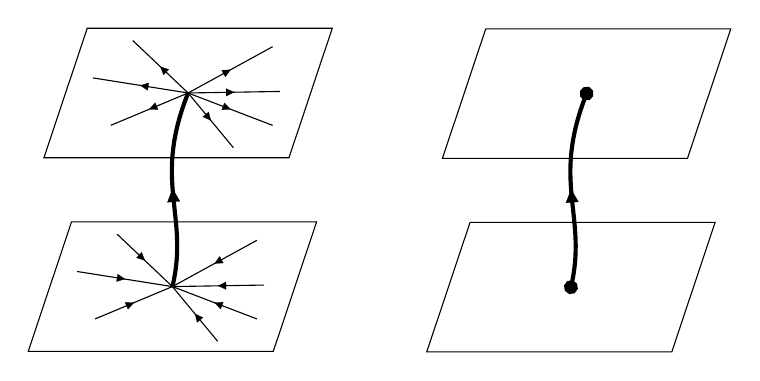
\begin{tikzpicture}[x=0.75pt,y=0.75pt,yscale=-0.6,xscale=0.6]

%Curve Lines [id:da8302434049369163] 
\draw [line width=1.5]    (142.8,220.53) .. controls (156.54,162.74) and (126.62,137.15) .. (155.4,65.07) ;
\draw [shift={(142.93,142)}, rotate = 445.15] [fill=black][line width=0.08] (10.45,-5.02) -- (0,0) -- (10.45,5.02) -- cycle    ;
%Straight Lines [id:da23152433957140084] 
\draw (155.4,65.07) -- (223.27,91.07) ;
\draw [shift={(189.34,78.07)}, rotate = 200.96] [fill=black][line width=0.08] (6.25,-3) -- (0,0) -- (6.25,3) -- cycle    ;
%Straight Lines [id:da7521717768429035] 
\draw (155.4,65.07) -- (223.27,27.9) ;
\draw [shift={(189.34,46.48)}, rotate = 511.3] [fill=black][line width=0.08] (6.25,-3) -- (0,0) -- (6.25,3) -- cycle    ;
%Straight Lines [id:da3813203099802065] 
\draw (78.93,52.95) -- (155.4,65.07) ;
\draw [shift={(117.17,59.01)}, rotate = 9] [fill=black][line width=0.08] (6.25,-3) -- (0,0) -- (6.25,3) -- cycle    ;
%Straight Lines [id:da7123700488843085] 
\draw (111.01,23) -- (155.4,65.07) ;
\draw [shift={(133.2,44.03)}, rotate = 43.46] [fill=black][line width=0.08] (6.25,-3) -- (0,0) -- (6.25,3) -- cycle    ;
%Straight Lines [id:da03896854735361477] 
\draw (93.25,91.07) -- (155.4,65.07) ;
\draw [shift={(124.33,78.07)}, rotate = 337.3] [fill=black][line width=0.08] (6.25,-3) -- (0,0) -- (6.25,3) -- cycle    ;
%Straight Lines [id:da9329409978551189] 
\draw (155.4,65.07) -- (229,63.84) ;
\draw [shift={(192.2,64.45)}, rotate = 539.05] [fill=black][line width=0.08] (6.25,-3) -- (0,0) -- (6.25,3) -- cycle    ;
%Straight Lines [id:da610320029346342] 
\draw (155.4,65.07) -- (191.77,109.04) ;
\draw [shift={(173.58,87.05)}, rotate = 230.4] [fill=black][line width=0.08] (6.25,-3) -- (0,0) -- (6.25,3) -- cycle    ;
%Straight Lines [id:da7334778053588917] 
\draw (142.8,220.53) -- (210.67,246.53) ;
\draw [shift={(176.73,233.53)}, rotate = 20.96] [fill=black][line width=0.08] (6.25,-3) -- (0,0) -- (6.25,3) -- cycle    ;
%Straight Lines [id:da9378344826057308] 
\draw (142.8,220.53) -- (210.67,183.36) ;
\draw [shift={(176.73,201.95)}, rotate = 331.3] [fill=black][line width=0.08] (6.25,-3) -- (0,0) -- (6.25,3) -- cycle    ;
%Straight Lines [id:da9881097931142797] 
\draw (66.33,208.41) -- (142.8,220.53) ;
\draw [shift={(104.57,214.47)}, rotate = 189] [fill=black][line width=0.08] (6.25,-3) -- (0,0) -- (6.25,3) -- cycle    ;
%Straight Lines [id:da4582833618389974] 
\draw (98.41,178.46) -- (142.8,220.53) ;
\draw [shift={(120.6,199.5)}, rotate = 223.46] [fill=black][line width=0.08] (6.25,-3) -- (0,0) -- (6.25,3) -- cycle    ;
%Straight Lines [id:da8348848056585603] 
\draw (80.65,246.53) -- (142.8,220.53) ;
\draw [shift={(111.73,233.53)}, rotate = 517.3] [fill=black][line width=0.08] (6.25,-3) -- (0,0) -- (6.25,3) -- cycle    ;
%Straight Lines [id:da08880361463986741] 
\draw (142.8,220.53) -- (216.4,219.3) ;
\draw [shift={(179.6,219.92)}, rotate = 359.05] [fill=black][line width=0.08] (6.25,-3) -- (0,0) -- (6.25,3) -- cycle    ;
%Straight Lines [id:da8383003573879682] 
\draw (142.8,220.53) -- (179.17,264.5) ;
\draw [shift={(160.98,242.51)}, rotate = 50.4] [fill=black][line width=0.08] (6.25,-3) -- (0,0) -- (6.25,3) -- cycle    ;
%Shape: Parallelogram [id:dp246128323677548] 
\draw (74.4,13.07) -- (271.17,13.07) -- (236.4,117.07) -- (39.62,117.07) -- cycle ;
%Shape: Parallelogram [id:dp8791964421429035] 
\draw (61.79,168.53) -- (258.57,168.53) -- (223.8,272.53) -- (27.02,272.53) -- cycle ;
%Curve Lines [id:da06968415810535933] 
\draw [line width=1.5]    (462.8,221) .. controls (476.54,163.21) and (446.62,137.62) .. (475.4,65.54) ;
\draw [shift={(475.4,65.54)}, rotate = 291.77][fill=black][line width=1.5]      (0, 0) circle [x radius= 3.92, y radius= 3.92]   ;
\draw [shift={(462.93,142.47)}, rotate = 445.15] [fill=black][line width=0.08] (10.45,-5.02) -- (0,0) -- (10.45,5.02) -- cycle    ;
\draw [shift={(462.8,221)}, rotate = 283.38][fill=black][line width=1.5]      (0, 0) circle [x radius= 3.92, y radius= 3.92]   ;
%Shape: Parallelogram [id:dp7681509431387952] 
\draw (394.4,13.54) -- (591.17,13.54) -- (556.4,117.54) -- (359.62,117.54) -- cycle ;
%Shape: Parallelogram [id:dp4460236924384613] 
\draw (381.79,169) -- (578.57,169) -- (543.8,273) -- (347.02,273) -- cycle ;

\end{tikzpicture}

\caption{Representation in one dimension less of the typical structure of ``monopole currents'' and ``vortex currents'' in 2-point correlators}
\label{eq:locality-monopole-vortex}
\end{figure}

One can almost rigorously prove that for $e^2$ large enough (strong coupling limit) the monopole quantum field operator $\op M(\vec x)$ couple the vacuum $\ket0$ to a 1-particle state together with an infrared Coulomb tail (called \emph{one-infraparticle state}\footnote{One cannot think about such state as a pole of the Green function, since the mass hyperboloid associated to the monopole interacts with the rest for the froward light cone, due to the presence of the field $E^x$, so that the pole of the Green function is blurred by the photon. This cannot be proved perturbatively, but using the non-perturbative Bloch-Nordsieck treatment.}), hence $\op M(\vec x)$ creates and annihilates monopole infra-particles. 

Furthermore the mass of the monopole turns out to be $O(e^2)$, hence, similarly to the case of vortices, monopole correlators with non-vanishing total monopole charge vanish, so that the Hilbert space of states of electrodynamic with monopoles for large $e^2$ develops monopole superselection sectors $\hs_q$ labelled by the total magnetic charge. Therefore the total Hilbert space of the theory is given by
\begin{eq}
	\hs=\bigoplus_{q\in\Z}\hs_q
\end{eq}
with
\begin{eq}
	\op M^\dagger \,:\,\hs_q\to\hs_{q+1}
\end{eq}
Conversely to the case $e^2\gg1$, where opening a closed defect ``costs a lot'', for $e^2$ small enough (weak coupling limit) the monopole ``condense'', i.e. there is a huge amount of open line defects in the partition function, and such defects ``hides'' the monopoles, so that $\hs=\hs_0$. 

\section{Spin ice}

\cite{Castelnovo:2008aa}\\

Although Dirac monopoles have not been found as elementary particles, and in fact they suffer of an UV problem, in 2008 a kind of exotic magnets called \emph{spin ice} have been studied, in which there seems to appear excitations similar to Dirac monopoles.\footnote{Original work: \cite{Castelnovo:2008aa}.}  The name comes from the fact that their structure is reminiscent of that of the ice. 

The structure appearing in the portion of oxygen and hydrogen in ice is tetrahedral, as represented in fig.~\ref{fig:ice}.
%
\begin{figure}[h]
\centering



\tikzset{every picture/.style={line width=0.75pt}} %set default line width to 0.75pt        

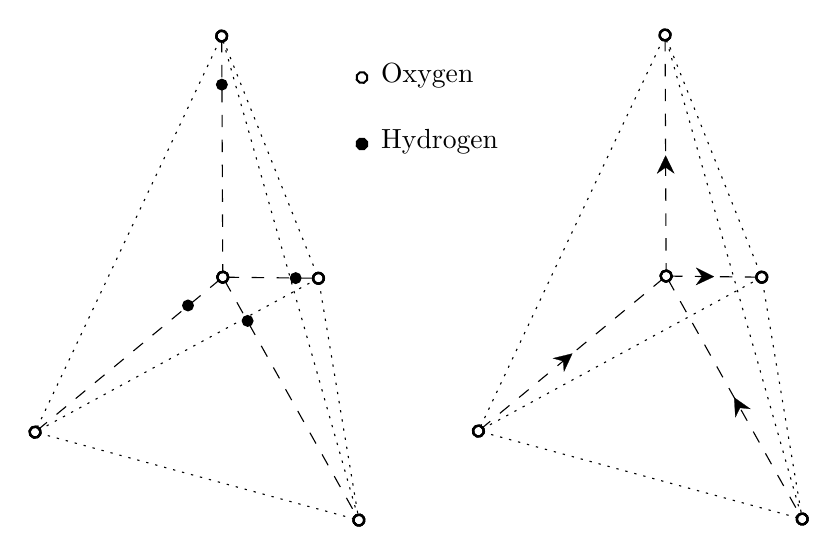
\begin{tikzpicture}[x=0.75pt,y=0.75pt,yscale=-0.8,xscale=0.8]
%uncomment if require: \path (0,300); %set diagram left start at 0, and has height of 300

%Straight Lines [id:da7779340734598339] 
\draw [dash pattern={on 0.84pt off 2.51pt}]  (195.4,8.31) -- (85,242.55) ;
\draw [shift={(84,244.68)}, rotate = 115.24][line width=0.75]      (0, 0) circle [x radius= 3.35, y radius= 3.35]   ;
\draw [shift={(196.41,6.19)}, rotate = 115.24][line width=0.75]      (0, 0) circle [x radius= 3.35, y radius= 3.35]   ;
%Straight Lines [id:da2094013016890539] 
\draw [dash pattern={on 0.84pt off 2.51pt}]  (197.28,8.37) -- (253.8,149.83) ;
\draw [shift={(254.67,152.01)}, rotate = 68.22][line width=0.75]      (0, 0) circle [x radius= 3.35, y radius= 3.35]   ;
\draw [shift={(196.41,6.19)}, rotate = 68.22][line width=0.75]      (0, 0) circle [x radius= 3.35, y radius= 3.35]   ;
%Straight Lines [id:da22391521746858856] 
\draw [dash pattern={on 0.84pt off 2.51pt}]  (278.36,295.39) -- (197.05,8.45) ;
\draw [shift={(196.41,6.19)}, rotate = 254.18][line width=0.75]      (0, 0) circle [x radius= 3.35, y radius= 3.35]   ;
\draw [shift={(279,297.65)}, rotate = 254.18][line width=0.75]      (0, 0) circle [x radius= 3.35, y radius= 3.35]   ;
%Straight Lines [id:da7440698596174549] 
\draw [dash pattern={on 4.5pt off 4.5pt}]  (196.42,8.54) -- (197.05,149.01) ;
\draw [shift={(197.06,151.36)}, rotate = 89.74][line width=0.75]      (0, 0) circle [x radius= 3.35, y radius= 3.35]   ;
\draw [shift={(196.41,6.19)}, rotate = 89.74][line width=0.75]      (0, 0) circle [x radius= 3.35, y radius= 3.35]   ;
%Straight Lines [id:da12830230249803742] 
\draw [dash pattern={on 4.5pt off 4.5pt}]  (195.25,152.85) -- (85.81,243.18) ;
\draw [shift={(84,244.68)}, rotate = 140.46][line width=0.75]      (0, 0) circle [x radius= 3.35, y radius= 3.35]   ;
\draw [shift={(197.06,151.36)}, rotate = 140.46][line width=0.75]      (0, 0) circle [x radius= 3.35, y radius= 3.35]   ;
%Straight Lines [id:da10677579926867731] 
\draw [dash pattern={on 4.5pt off 4.5pt}]  (198.21,153.41) -- (277.85,295.6) ;
\draw [shift={(279,297.65)}, rotate = 60.75][line width=0.75]      (0, 0) circle [x radius= 3.35, y radius= 3.35]   ;
\draw [shift={(197.06,151.36)}, rotate = 60.75][line width=0.75]      (0, 0) circle [x radius= 3.35, y radius= 3.35]   ;
%Straight Lines [id:da08291812818968824] 
\draw [dash pattern={on 4.5pt off 4.5pt}]  (199.41,151.38) -- (252.32,151.98) ;
\draw [shift={(254.67,152.01)}, rotate = 0.65][line width=0.75]      (0, 0) circle [x radius= 3.35, y radius= 3.35]   ;
\draw [shift={(197.06,151.36)}, rotate = 0.65][line width=0.75]      (0, 0) circle [x radius= 3.35, y radius= 3.35]   ;
%Straight Lines [id:da8215533424387143] 
\draw [dash pattern={on 0.84pt off 2.51pt}]  (86.27,245.3) -- (276.73,297.04) ;
\draw [shift={(279,297.65)}, rotate = 15.2][line width=0.75]      (0, 0) circle [x radius= 3.35, y radius= 3.35]   ;
\draw [shift={(84,244.68)}, rotate = 15.2][line width=0.75]      (0, 0) circle [x radius= 3.35, y radius= 3.35]   ;
%Straight Lines [id:da32221379808607975] 
\draw [dash pattern={on 0.84pt off 2.51pt}]  (86.07,243.56) -- (252.6,153.13) ;
\draw [shift={(254.67,152.01)}, rotate = 331.5][line width=0.75]      (0, 0) circle [x radius= 3.35, y radius= 3.35]   ;
\draw [shift={(84,244.68)}, rotate = 331.5][line width=0.75]      (0, 0) circle [x radius= 3.35, y radius= 3.35]   ;
%Straight Lines [id:da9880502250610932] 
\draw [dash pattern={on 0.84pt off 2.51pt}]  (255.06,154.33) -- (278.61,295.33) ;
\draw [shift={(279,297.65)}, rotate = 80.52][line width=0.75]      (0, 0) circle [x radius= 3.35, y radius= 3.35]   ;
\draw [shift={(254.67,152.01)}, rotate = 80.52][line width=0.75]      (0, 0) circle [x radius= 3.35, y radius= 3.35]   ;
%Shape: Circle [id:dp4408572844254719] 
\draw [fill=black,fill opacity=1 ] (208.75,177.7) .. controls (208.75,175.91) and (210.21,174.45) .. (212,174.45) .. controls (213.79,174.45) and (215.25,175.91) .. (215.25,177.7) .. controls (215.25,179.49) and (213.79,180.95) .. (212,180.95) .. controls (210.21,180.95) and (208.75,179.49) .. (208.75,177.7) -- cycle ;
%Shape: Circle [id:dp8591579522801442] 
\draw [fill=black,fill opacity=1 ] (237.7,151.92) .. controls (237.7,150.13) and (239.16,148.67) .. (240.95,148.67) .. controls (242.75,148.67) and (244.2,150.13) .. (244.2,151.92) .. controls (244.2,153.72) and (242.75,155.17) .. (240.95,155.17) .. controls (239.16,155.17) and (237.7,153.72) .. (237.7,151.92) -- cycle ;
%Shape: Circle [id:dp9270340091397358] 
\draw [fill=black,fill opacity=1 ] (193.25,35.4) .. controls (193.25,33.61) and (194.71,32.15) .. (196.5,32.15) .. controls (198.29,32.15) and (199.75,33.61) .. (199.75,35.4) .. controls (199.75,37.19) and (198.29,38.65) .. (196.5,38.65) .. controls (194.71,38.65) and (193.25,37.19) .. (193.25,35.4) -- cycle ;
%Shape: Circle [id:dp42417247389203117] 
\draw [fill=black,fill opacity=1 ] (172.85,168.4) .. controls (172.85,166.61) and (174.31,165.15) .. (176.1,165.15) .. controls (177.89,165.15) and (179.35,166.61) .. (179.35,168.4) .. controls (179.35,170.19) and (177.89,171.65) .. (176.1,171.65) .. controls (174.31,171.65) and (172.85,170.19) .. (172.85,168.4) -- cycle ;
%Straight Lines [id:da7591368397307141] 
\draw [dash pattern={on 0.84pt off 2.51pt}]  (462.4,7.66) -- (352,241.9) ;
\draw [shift={(351,244.03)}, rotate = 115.24][line width=0.75]      (0, 0) circle [x radius= 3.35, y radius= 3.35]   ;
\draw [shift={(463.41,5.54)}, rotate = 115.24][line width=0.75]      (0, 0) circle [x radius= 3.35, y radius= 3.35]   ;
%Straight Lines [id:da3444542785016118] 
\draw [dash pattern={on 0.84pt off 2.51pt}]  (464.28,7.72) -- (520.8,149.18) ;
\draw [shift={(521.67,151.36)}, rotate = 68.22][line width=0.75]      (0, 0) circle [x radius= 3.35, y radius= 3.35]   ;
\draw [shift={(463.41,5.54)}, rotate = 68.22][line width=0.75]      (0, 0) circle [x radius= 3.35, y radius= 3.35]   ;
%Straight Lines [id:da3886783094945634] 
\draw [dash pattern={on 0.84pt off 2.51pt}]  (545.36,294.74) -- (464.05,7.8) ;
\draw [shift={(463.41,5.54)}, rotate = 254.18][line width=0.75]      (0, 0) circle [x radius= 3.35, y radius= 3.35]   ;
\draw [shift={(546,297)}, rotate = 254.18][line width=0.75]      (0, 0) circle [x radius= 3.35, y radius= 3.35]   ;
%Straight Lines [id:da295775823341778] 
\draw [dash pattern={on 4.5pt off 4.5pt}]  (463.42,7.89) -- (464.05,148.35) ;
\draw [shift={(464.06,150.7)}, rotate = 89.74][line width=0.75]      (0, 0) circle [x radius= 3.35, y radius= 3.35]   ;
\draw [shift={(463.73,78.12)}, rotate = 89.74] [fill=black][line width=0.08] (10.72,-5.15) -- (0,0) -- (10.72,5.15) -- (7.12,0) -- cycle    ;
\draw [shift={(463.41,5.54)}, rotate = 89.74][line width=0.75]      (0, 0) circle [x radius= 3.35, y radius= 3.35]   ;
%Straight Lines [id:da7853830909468005] 
\draw [dash pattern={on 4.5pt off 4.5pt}]  (462.25,152.2) -- (352.81,242.53) ;
\draw [shift={(351,244.03)}, rotate = 140.46][line width=0.75]      (0, 0) circle [x radius= 3.35, y radius= 3.35]   ;
\draw [shift={(407.53,197.37)}, rotate = 140.46] [fill=black][line width=0.08] (10.72,-5.15) -- (0,0) -- (10.72,5.15) -- (7.12,0) -- cycle    ;
\draw [shift={(464.06,150.7)}, rotate = 140.46][line width=0.75]      (0, 0) circle [x radius= 3.35, y radius= 3.35]   ;
%Straight Lines [id:da027134956928842158] 
\draw [dash pattern={on 4.5pt off 4.5pt}]  (465.21,152.75) -- (544.85,294.95) ;
\draw [shift={(546,297)}, rotate = 60.75][line width=0.75]      (0, 0) circle [x radius= 3.35, y radius= 3.35]   ;
\draw [shift={(505.03,223.85)}, rotate = 60.75] [fill=black][line width=0.08] (10.72,-5.15) -- (0,0) -- (10.72,5.15) -- (7.12,0) -- cycle    ;
\draw [shift={(464.06,150.7)}, rotate = 60.75][line width=0.75]      (0, 0) circle [x radius= 3.35, y radius= 3.35]   ;
%Straight Lines [id:da17976783307978605] 
\draw [dash pattern={on 4.5pt off 4.5pt}]  (466.41,150.73) -- (519.32,151.33) ;
\draw [shift={(521.67,151.36)}, rotate = 0.65][line width=0.75]      (0, 0) circle [x radius= 3.35, y radius= 3.35]   ;
\draw [shift={(492.87,151.03)}, rotate = 180.65] [fill=black][line width=0.08] (10.72,-5.15) -- (0,0) -- (10.72,5.15) -- (7.12,0) -- cycle    ;
\draw [shift={(464.06,150.7)}, rotate = 0.65][line width=0.75]      (0, 0) circle [x radius= 3.35, y radius= 3.35]   ;
%Straight Lines [id:da9878093991830288] 
\draw [dash pattern={on 0.84pt off 2.51pt}]  (353.27,244.64) -- (543.73,296.38) ;
\draw [shift={(546,297)}, rotate = 15.2][line width=0.75]      (0, 0) circle [x radius= 3.35, y radius= 3.35]   ;
\draw [shift={(351,244.03)}, rotate = 15.2][line width=0.75]      (0, 0) circle [x radius= 3.35, y radius= 3.35]   ;
%Straight Lines [id:da3384465595014927] 
\draw [dash pattern={on 0.84pt off 2.51pt}]  (353.07,242.91) -- (519.6,152.48) ;
\draw [shift={(521.67,151.36)}, rotate = 331.5][line width=0.75]      (0, 0) circle [x radius= 3.35, y radius= 3.35]   ;
\draw [shift={(351,244.03)}, rotate = 331.5][line width=0.75]      (0, 0) circle [x radius= 3.35, y radius= 3.35]   ;
%Straight Lines [id:da9910775832584819] 
\draw [dash pattern={on 0.84pt off 2.51pt}]  (522.06,153.68) -- (545.61,294.68) ;
\draw [shift={(546,297)}, rotate = 80.52][line width=0.75]      (0, 0) circle [x radius= 3.35, y radius= 3.35]   ;
\draw [shift={(521.67,151.36)}, rotate = 80.52][line width=0.75]      (0, 0) circle [x radius= 3.35, y radius= 3.35]   ;

\draw [shift={(280.86,31.14)}, rotate = 68.22][line width=0.75]      (0, 0) circle [x radius= 3.35, y radius= 3.35]   ;
\draw [shift={(280.86,71.14)}, rotate = 68.22][fill=black,fill opacity=1 ] [line width=0.75]      (0, 0) circle [x radius= 3.35, y radius= 3.35]   ;

 

% Text Node
\draw (290.86,21.14) node [anchor=north west][inner sep=0.75pt]   [align=left] {Oxygen\\\\Hydrogen};


\end{tikzpicture}

\caption{Tetrahedral structure of the ice: one oxygen is connected to other oxygens along the direction of a tetrahedron, and in between two oxygens there is an hydrogen. However of these four hydrogens contained in the tetrahedron two are nearer to the central oxygen and their bounds are covariant, and two are more far, and their bounds are of hydrogen type. In the second picture we represented the positions of the hydrogens by means of displacement vectors, pointing in the direction of the displacement of the hydrogen atom with respect to the center of the bound. Hence in a tetrahedron two displacement vectors are inword and two are outword.}
\label{fig:ice}
\end{figure}

In spin ice materials the hydrogen is replaced is replaced by rare-earth ions and the displacement vector is replaced by a spin vector, each spin vector has only one possible direction and two possible orientations, i.e. Ising-like spins, along the bound. 

The Hamiltonian can be taken as 
\begin{eq}
	H=-J\sum_{\langle i,j\rangle}\vec S_i^{\hat z_i}\cdot\vec S_j^{\hat z_j}+D\sum_{i,j}\left[\frac{\vec S_i^{\hat z_i}\cdot\vec S_j^{\hat z_j}}{ r_{ij}^3}-3\frac{(\vec S_i^{\hat z_i}\cdot \vec r_{ij})(\vec S^{\op z_j}\cdot\vec r_{ij})}{ r_{ij}^5}\right]
\end{eq}
where $\vec S_i^{\op z_i}$ is the spin along the $\hat z_i$ radial direction from the center of the tetrahedron towards its vertex labelled by the site $i$, $\vec r_{ij}$ is the vector connecting the site $i$ and the site $j$. Furthermore the orientation of the spins in the first term are favouring the combination 2-in/2-out for each tetrahedron, as this is the minimal energy configuration. Indeed, since the angle $\theta$ between bounds give $\cos\theta=-\frac13$, we get the following energy contributions for the short range interaction:
\begin{eq}\begin{cases}
	\displaystyle\cenergy(\text{2 in, 2 out})=-2\frac J3S^2\\[0.7em] 
	\displaystyle\cenergy(\text{1 in, 3 out})=\cenergy(\text{3 in, 1 out})=0\frac J3S^2 \\[0.7em]
	\displaystyle\cenergy(\text{0 in, 4 out})=\cenergy(\text{4 in, 0 out})=2\frac J3S^2
\end{cases}\end{eq}
Notice that the minimal energy configuration 2-in/2-out is highly degenerate. 
The long-range part of the Hamiltonian is reminiscent of the dipolar interaction. Indeed the potential of a dipole $\vec p=q\vec d$ is 
\begin{eq}
	\phi(\vec x)=\frac{\vec p\cdot\vec x}{|\vec x|^3}
\end{eq}
where $q$ is the charge and $\vec d$ is the vector connecting the two charges of the dipole, and at large distances the potential energy of two interacting dipoles $\vec p_1$ and $\vec p_2$ in electrodynamics is given up to a sign by the scalar product between one of the dipoles and the electric field generated by the other one. 
Therefore if we call $\vec r$ the vector from $\vec p_1$ to $\vec p_2$ and $r:=|\vec r|$ then the energy of the dipolar interaction reads
\begin{eq}
	\cenergy=\vec p_1\cdot\vec\nabla\phi_2(\vec r)=\vec p_1\cdot\left(\frac{\vec p_2}{ r^3}-3\frac{(\vec r\cdot\vec p_2)\vec x}{r^5}\right)
	=\frac{\vec p_i\cdot\vec p_2}{r^3}-3\frac{(\vec r\cdot\vec p_1)(\vec r\cdot\vec p_2)}{r^5}
\end{eq}

Therefore we can replace the spins in the spin ice by dipoles ``at the end of the spin vectors'', so that the $+$ charge corresponds to the tail of the spin vector and the $-$ charge to its head, and such charges interact via Coulomb potential. It is natural to think of these charges as magnetic charges since the spin is naturally related to magnetism. In this way at the center of each tetrahedron the nearer charges of the 4 dipoles accumulate. More precisely, if the site center of the tetrahedron is labelled by $i$ we have for its charge
\begin{eq}
	Q_i=q_{i1}+q_{i2}+q_{i3}+q_{i4}
\end{eq}
where $q_{i\ell}$ is the charge of the $\ell$-th dipole which is closer to the site $i$. Charges of the centers interact via Coulomb interaction
\begin{eq}\label{eq:Coulomb}
	V=\frac{Q_iQ_j}{r_{ij}}
\end{eq}
Imposing an onsite energy $v_0\sum_i Q_i^2$, so that $Q_i=0$ on the ground state, enforces the ice rule, that is the configuration 2 in/2 out for each tetrahedron, as in the case of fig.~\ref{fig:spin-ice-dipole}. 

\begin{figure}[h]
\centering

\tikzset{every picture/.style={line width=0.75pt}} %set default line width to 0.75pt        
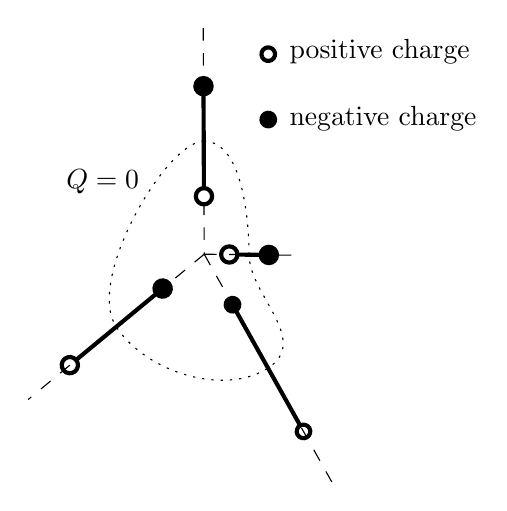
\begin{tikzpicture}[x=0.75pt,y=0.75pt,yscale=-0.75,xscale=0.75]

%Straight Lines [id:da973693891465115] 
\draw [dash pattern={on 4.5pt off 4.5pt}]  (175.41,6.54) -- (176.06,151.7) ;
%Straight Lines [id:da16774706075400037] 
\draw [dash pattern={on 4.5pt off 4.5pt}]  (176.06,151.7) -- (63,245.03) ;
%Straight Lines [id:da7656517139199785] 
\draw [dash pattern={on 4.5pt off 4.5pt}]  (176.06,151.7) -- (258,298) ;
%Straight Lines [id:da06940031014704706] 
\draw [dash pattern={on 4.5pt off 4.5pt}]  (176.06,151.7) -- (233.67,152.36) ;
%Straight Lines [id:da27365231738136764] 
\draw [line width=1.5]    (175.58,43.77) -- (175.87,110.25) ;
\draw [shift={(175.89,114.47)}, rotate = 89.75][line width=1.5]      (0, 0) circle [x radius= 5.23, y radius= 5.23]   ;
\draw [shift={(175.58,43.77)}, rotate = 89.75][fill=black][line width=1.5]      (0, 0) circle [x radius= 5.23, y radius= 5.23]   ;
%Straight Lines [id:da6738627227445009] 
\draw [line width=1.5]    (196.39,151.94) -- (217.57,152.18) ;
\draw [shift={(217.57,152.18)}, rotate = 0.65][fill=black][line width=1.5]      (0, 0) circle [x radius= 5.23, y radius= 5.23]   ;
\draw [shift={(192.16,151.89)}, rotate = 0.65][line width=1.5]      (0, 0) circle [x radius= 5.23, y radius= 5.23]   ;
%Straight Lines [id:da5182178087232998] 
\draw [line width=1.5]    (149.33,173.77) -- (92.99,220.27) ;
\draw [shift={(89.73,222.97)}, rotate = 140.46][line width=1.5]      (0, 0) circle [x radius= 5.23, y radius= 5.23]   ;
\draw [shift={(149.33,173.77)}, rotate = 140.46][fill=black][line width=1.5]      (0, 0) circle [x radius= 5.23, y radius= 5.23]   ;
%Straight Lines [id:da04996416143259297] 
\draw [line width=1.5]    (194.23,184.15) -- (238.19,262.63) ;
\draw [shift={(239.83,265.55)}, rotate = 60.75][line width=1.5]      (0, 0) circle [x radius= 4.36, y radius= 4.36]   ;
\draw [shift={(194.23,184.15)}, rotate = 60.75][fill=black][line width=1.5]      (0, 0) circle [x radius= 4.36, y radius= 4.36]   ;
%Shape: Polygon Curved [id:ds026298236726155277] 
\draw [dash pattern={on 0.84pt off 2.51pt}] (175.73,79.12) .. controls (199.8,79) and (204.73,126.26) .. (204.87,152.03) .. controls (205,177.8) and (244.6,207) .. (217.03,224.85) .. controls (189.46,242.7) and (139.53,228.37) .. (119.53,198.37) .. controls (99.53,168.37) and (151.67,79.24) .. (175.73,79.12) -- cycle ;

\draw [shift={(217.2,23.2)}, rotate = 60.75][line width=1.5]      (0, 0) circle [x radius= 4.36, y radius= 4.36]   ;
\draw [shift={(217.2,65.2)}, rotate = 60.75][fill=black][line width=1.5]      (0, 0) circle [x radius= 4.36, y radius= 4.36]   ;

% Text Node
\draw (85.8,95.6) node [anchor=north west][inner sep=0.75pt]   [align=left] {$\displaystyle Q=0$};
\draw (229.2,12.2) node [anchor=north west][inner sep=0.75pt]   [align=left] {positive charge\\\\negative charge};

\end{tikzpicture}

\caption{The tetrahedral cell of spin ice in the ``dipole'' representation, in the minimal energy configuration (2 in-2 out). Notice that in the region close to the center of the tetrahedron the total charge is $Q=1+1-1-1=0$.}
\label{fig:spin-ice-dipole}
\end{figure}

If we flip a spin, in one of the two tetrahedrons connected by that spin the total charge become 2, and in the other one become $-2$. The defects in the partition function of the model correspond to chains of spin flips. If a site is intermediate between two spin flips cleverly chosen, then two opposite charges of that site in the dipole picture have changed their signs, so we still have $Q=0$ in that site. However at the ends of a chain of spin flips we have 3 charges of the same sign and one with the opposite one, so that $Q\neq0$. Since these charges interact according to the Coulomb interaction eq.~\eqref{eq:Coulomb}, they can be interpreted as monopoles. Therefore at each end of a chain of spin flips we have a ``magnetic monopole'' if $Q>0$ of a ``magnetic antimonopole'' if $Q<0$. The string of spin flips is nothing but a ``Dirac string''. Such situation is represented in fig.~\ref{fig:spin-flips}

\begin{figure}[h]
\centering

\tikzset{every picture/.style={line width=0.75pt}} %set default line width to 0.75pt        
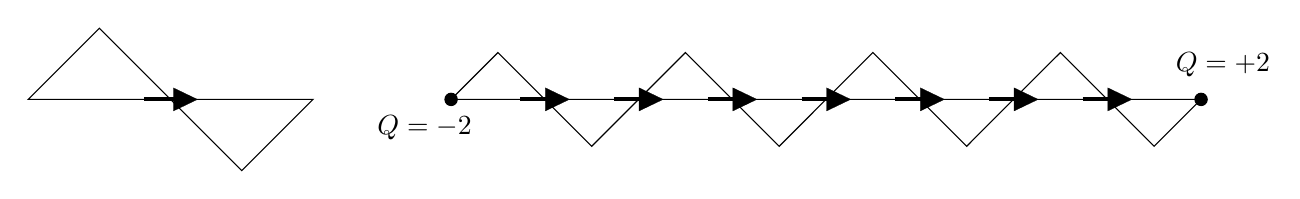
\begin{tikzpicture}[x=0.75pt,y=0.75pt,yscale=-1,xscale=1]
%uncomment if require: \path (0,300); %set diagram left start at 0, and has height of 300

%Shape: Polygon [id:ds3373611249685007] 
\draw (60.9,105.8) -- (95.2,140.1) -- (129.5,174.4) -- (163.8,140.1) -- (26.6,140.1) -- cycle ;
%Straight Lines [id:da567703536540205] 
\draw [line width=1.5]    (82.26,140.1) -- (104.14,140.1) ;
\draw [shift={(108.14,140.1)}, rotate = 180] [fill=black][line width=0.08] (11.61,-5.58) -- (0,0) -- (11.61,5.58) -- cycle    ;
%Shape: Polygon [id:ds4302598258410022] 
\draw (252.92,117.5) -- (275.5,140.08) -- (298.08,162.67) -- (320.67,140.08) -- (230.33,140.08) -- cycle ;
%Straight Lines [id:da7575750767564635] 
\draw [line width=1.5]    (263.66,140.08) -- (283.34,140.08) ;
\draw [shift={(287.34,140.08)}, rotate = 180] [fill=black][line width=0.08] (11.61,-5.58) -- (0,0) -- (11.61,5.58) -- cycle    ;
%Shape: Polygon [id:ds7760452095741674] 
\draw (343.25,117.5) -- (365.83,140.08) -- (388.42,162.67) -- (411,140.08) -- (320.67,140.08) -- cycle ;
%Shape: Polygon [id:ds19799972468632188] 
\draw (433.58,117.5) -- (456.17,140.08) -- (478.75,162.67) -- (501.33,140.08) -- (411,140.08) -- cycle ;
%Shape: Polygon [id:ds2643613467242225] 
\draw (523.92,117.5) -- (546.5,140.08) -- (569.08,162.67) -- (591.67,140.08) -- (501.33,140.08) -- cycle ;
%Straight Lines [id:da48819086642356235] 
\draw [line width=1.5]    (308.82,140.08) -- (328.51,140.08) ;
\draw [shift={(332.51,140.08)}, rotate = 180] [fill=black][line width=0.08] (11.61,-5.58) -- (0,0) -- (11.61,5.58) -- cycle    ;
%Straight Lines [id:da14801558177916063] 
\draw [line width=1.5]    (353.99,140.08) -- (373.68,140.08) ;
\draw [shift={(377.68,140.08)}, rotate = 180] [fill=black][line width=0.08] (11.61,-5.58) -- (0,0) -- (11.61,5.58) -- cycle    ;
%Straight Lines [id:da7637986970069108] 
\draw [line width=1.5]    (399.16,140.08) -- (418.84,140.08) ;
\draw [shift={(422.84,140.08)}, rotate = 180] [fill=black][line width=0.08] (11.61,-5.58) -- (0,0) -- (11.61,5.58) -- cycle    ;
%Straight Lines [id:da5140113640305328] 
\draw [line width=1.5]    (444.32,140.08) -- (464.01,140.08) ;
\draw [shift={(468.01,140.08)}, rotate = 180] [fill=black][line width=0.08] (11.61,-5.58) -- (0,0) -- (11.61,5.58) -- cycle    ;
%Straight Lines [id:da13967326849119188] 
\draw [line width=1.5]    (489.49,140.08) -- (509.18,140.08) ;
\draw [shift={(513.18,140.08)}, rotate = 180] [fill=black][line width=0.08] (11.61,-5.58) -- (0,0) -- (11.61,5.58) -- cycle    ;
%Straight Lines [id:da5971180607342266] 
\draw [line width=1.5]    (534.66,140.08) -- (554.34,140.08) ;
\draw [shift={(558.34,140.08)}, rotate = 180] [fill=black][line width=0.08] (11.61,-5.58) -- (0,0) -- (11.61,5.58) -- cycle    ;
%Shape: Circle [id:dp441711292376024] 
\draw [fill=black,fill opacity=1 ] (227.37,140.08) .. controls (227.37,138.44) and (228.69,137.12) .. (230.33,137.12) .. controls (231.97,137.12) and (233.3,138.44) .. (233.3,140.08) .. controls (233.3,141.72) and (231.97,143.05) .. (230.33,143.05) .. controls (228.69,143.05) and (227.37,141.72) .. (227.37,140.08) -- cycle ;
%Shape: Circle [id:dp22948531046480758] 
\draw [fill=black,fill opacity=1 ] (588.7,140.08) .. controls (588.7,138.44) and (590.03,137.12) .. (591.67,137.12) .. controls (593.31,137.12) and (594.63,138.44) .. (594.63,140.08) .. controls (594.63,141.72) and (593.31,143.05) .. (591.67,143.05) .. controls (590.03,143.05) and (588.7,141.72) .. (588.7,140.08) -- cycle ;

% Text Node
\draw (193.6,146.6) node [anchor=north west][inner sep=0.75pt]    {$Q=-2$};
% Text Node
\draw (578.27,116.2) node [anchor=north west][inner sep=0.75pt]    {$Q=+2$};


\end{tikzpicture}

\caption{On the left, the two triangles represent two close tetrahedrons, and the arrow represent a flip of the spin shared between them. On the right, we have the representation of a chain of spin flips, chosen so that it represent a ``Dirac string'' whose boundaries constitute a ``monopole-antimonopole pair''. }
\label{fig:spin-flips}
\end{figure}

If we introduce the time dimension these configurations describes precisely worldlines of  virtual monopole-antimonopole pairs with a Dirac string between them spanning a surface bounded by that worldline. 

\section{Condensation of defects}

We close the discussion about solitons with a final remark about phase transitions. We have seen that quantum solitons correspond in their Euclidean description to line-defects. We also remarked that it may happen that line-defects reach $\infty$ with finite probability, i.e. they give raise to the phenomenon called \emph{condensation of defects}. When condensation of defects occurs the soliton sectors disappear. The transition from a situation where configurations allowed are only with finite defects (``dilute gas of defects'') to a situation where also infinitely extended defects appear corresponds to a \emph{phase transition}. 

\skipline

As we said, defects can have arbitrary dimension\footnote{Recall that the dimensin of the defect is the dimension of its locus, where the singularity appears.} $k$. We now show heuristically that for $k>0$ condensation of defects is a general mechanism of phase transition. Suppose for simplicity that only one species of defects appears in the model under consideration, but the extension to multiple species is straightforward. 

For $k>0$ the mean action $\bar S$ of a $k$-dimensional defect $D^k$ is typically proportional to the volume of the locus of $D^k$, i.e.
\begin{eq}
	\bar S(D^k)\sim c_k\beta|D^k|
\end{eq}
where $\beta$ is the relevant coupling constant of the model, $c_k>0$ is a suitable constant and $|D^k|$ is the volume of the locus of the defect suitably discretized. 

The number of such defects containing a fixed point, say the origin, and with fixed discretized volume $|D^k|$, is bounded by $\lexp{d_k|D^k|}$, for some constant $d_k>0$. To get a hint of this bound consider the simplest case of a line defect in dimension $d=2$. Consider a kink containing the origin, since we are considering a discretized space, it is trivial to notice that the first ``piece'' of the kink can be chosen is $2d$ ways, since there are $2d$ possible locus around the origin which can be connected with the origin itself. Then we may add another ``piece'' of kink in $2d-1$ ways, as we cannot ``go back'', and the same is true for all other ``pieces'',\footnote{Actually, in some cases it may happen that we have less than $2d-1$ possible choices, as otherwise we get a closed defect, but we ignore this issue as we are looking for an higher bound to the number of possible defects.} obtaining in this way a line defect of dimension $L=|D^1|$ after $L-1$ steps. Hence there are at most 
\begin{eq}
	2d(2d-1)^{L-1}\leq \lexp{L\log 2d}
\end{eq}
line defects of length $L$ containing the origin, and this proves that for $k=1$ we have $d_1=\log 2d$. 

As discussed for the kink in $\phi_2^4$, one can write in general the partition function of the model with $k$-defects, denoted $D$ from now on for simplicity, as the partition function of an interacting gas of defects. Assuming that defects are weakly interacting we get from eq.~\eqref{eq:Zsc} that
\begin{eq}
	Z\approx\sum_{N=0}^\infty\ \sum_{\{D_1,\ldots,D_N\}}\ \prod_{i=1}^N\lexp{-\bar S(D_i)}
\end{eq}
Let's now consider the contribution to the partition function of the defects of volume $|D|$ containing the origin. By the esitmate above such contribution goes like
\begin{eq}
	\lexp{-\bar S(D)}\lexp{d_k|D|}\approx \lexp{(d_k-c_k\beta)|D|}
\end{eq}
We immediately see that for $|D|\to\infty$
\begin{eq}
	\lexp{(d_k-c_k\beta)|D|}
	\xrightarrow[|D|\to\infty]{}
	\begin{cases}
		0&\tif d_k-c_k\beta<0\\
		\infty&\tif d_k-c_k\beta>0
	\end{cases}
\end{eq}
The first case implies that there are no defects of infinite volume containing the origin (their Boltzmann weight vanish), the second case instead suggests that there are defects containing the origin reaching infinity with finite probability and that there is a critical value $\beta_c$ for $\beta$ where the transition occurs. 

One can heuristically interpret in this way the transition from the symmetry breaking phase to the unbroken phase in the case of kinks, from superconductors with massive photon to the usual Coulomb phase with massless photons in the case of vortices, and so on. 

Although this mechanism of phase transition is quite general, specific for the line defects is the related appearance of soliton sectors and usually of quantum soliton particles in the phase where the gas of defects is dilute, i.e. where there are no infinite-long defects. 

\end{document}